% Association for Computational Linguistics Rolling Review (ARR) long paper.
% Submission is to ARR via OpenReview (not directly to a venue). After review
% and meta-review, the same paper may be committed to a participating
% conference such as ACL 2026 according to that venue's deadlines. ARR
% long papers: up to 8 pages of main content plus unlimited References;
% Limitations section required before references and does not count toward
% the eight pages; Ethics / Ethical Considerations unlimited after Limitations.
% arXiv preprint version -- de-anonymized for public release.
% [preprint] keeps page numbers but removes line numbers and anonymization.
%
% Source of truth for the empirical claims is
% Guidance_Documents/study_design.md and the per-cell artefacts under
% divergence_study_outputs/. Update both in lockstep.

\documentclass[11pt]{article}

\usepackage[review]{acl}

\usepackage{times}
\usepackage{latexsym}
\usepackage[T1]{fontenc}
\usepackage[utf8]{inputenc}
\usepackage{microtype}
\usepackage{inconsolata}
\usepackage{graphicx}
\usepackage{booktabs}
\usepackage{amsmath}
\usepackage{amssymb}
\usepackage{mathtools}
\usepackage{xcolor}
\usepackage{tcolorbox}
\usepackage{tikz}
\usetikzlibrary{positioning, arrows.meta, calc, fit, shapes.geometric, backgrounds}
\usepackage{ifthen}

% Project-wide aquatic palette mirrored from scripts/figure_style.py: a single
% blue-green family across every figure, with no warm hues anywhere. Generic
% role names are kept so the TikZ hero file does not need to be retouched if
% individual shades are later retuned.
\definecolor{stdgrey}{HTML}{7E9AAB}      % cool blue-grey (standard CoT baseline)
\definecolor{ncotteal}{HTML}{0E7C7B}     % jewel teal (narration-of-thought)
\definecolor{ncottealdk}{HTML}{0A5C5B}   % darker teal (text accent on light teal)
\definecolor{vendorblue}{HTML}{2E7DA0}   % steel-teal (multi-agent role A)
\definecolor{vendorsienna}{HTML}{0E5C5B} % deep teal (multi-agent role B)
\definecolor{vendorplum}{HTML}{5BB0A8}   % sea green (multi-agent role C)
\definecolor{alarmred}{HTML}{1A3B6E}     % deep navy (failure indicators)
\definecolor{paleslate}{HTML}{E2EAF0}    % pale blue-grey
\definecolor{paleteal}{HTML}{D9ECEB}     % pale teal
\definecolor{paleblue}{HTML}{D6E5EE}     % pale steel-teal
\definecolor{palesienna}{HTML}{C9E1DC}   % pale deep-teal tint
\definecolor{paleplum}{HTML}{DCEEEB}     % pale sea-green
\definecolor{palealarm}{HTML}{C9D7E6}    % pale navy

\usepackage{multirow}
\usepackage{tabularx}
\usepackage{algorithm}
\usepackage{algpseudocode}
\usepackage{url}
% Long file paths in \path{} break at common separators.
\urlstyle{tt}
\DeclareUrlCommand\path{\urlstyle{tt}}


\title{Narration-of-Thought:\\
Inference-Time Scaffolding for Defeasible Ethical Reasoning\\
in Large Language Models}

\author{Anonymous ARR Submission}

\begin{document}
\maketitle

\begin{abstract}
Standard chain-of-thought (CoT) on moral dilemmas exhibits two
failure modes that matter for deployment: stakeholder collapse (the
reasoning trace names at most one party with a stake in the outcome)
and uncertainty suppression (the trace contains no explicit unknowns
or hedges before committing to an action). We introduce
narration-of-thought (NoT), a system prompt that constrains the trace
to five narrative sections: protagonist, stakeholders, two-step
consequences, uncertainty, and only then commitment. NoT adds no
training data, parameters, or fine-tuning. On a 100-scenario
DailyDilemmas sample across five models from four vendors, NoT cuts
stakeholder collapse from up to $30\%$ of traces to at most $1.2\%$
and uncertainty suppression from up to $71\%$ to $0$--$24\%$ on every
model. A
matched-budget verbose-CoT control rules out token spend as the
active ingredient, a section-by-section ablation attributes each
shift to the sub-instruction that carries it, and textual-gradient
descent initialised at NoT improves the scaffold further, with a
training judge from a different vendor than the generator beating a
same-vendor judge on every
measured axis. Extended to a five-round multi-stakeholder debate in
which three stakeholder agents vote on a moderator-integrated
proposal, the scaffold converts a $6\%$ standoff into $95\%$ full
consensus, with residual rejections concentrated in roles whose stake
the proposal materially undermines. The resulting traces externalise
the stakeholders, consequences, and uncertainty grounding each
commitment, providing an auditable substrate for dependable
agentic-workflow deployment.
\end{abstract}

\begin{figure*}[!t]
\centering
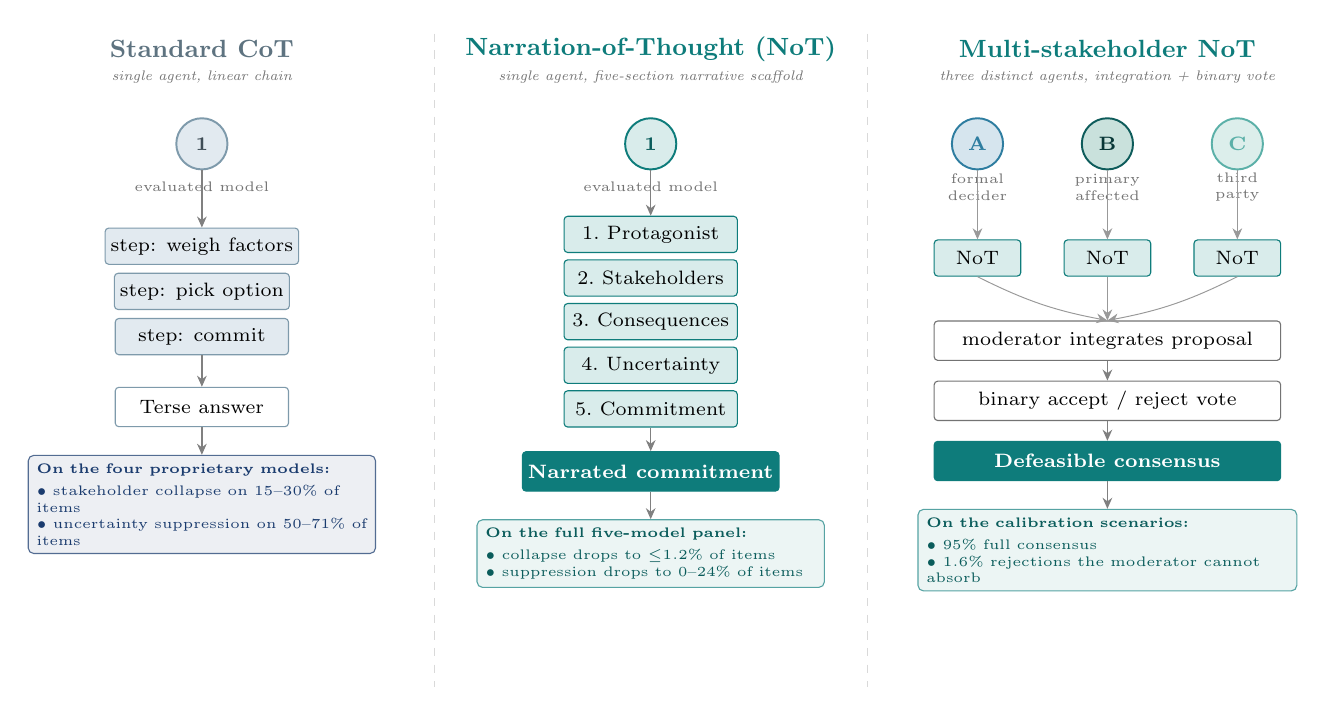
\begin{tikzpicture}[
  >={Stealth[length=4pt, width=3.5pt]},
  font=\footnotesize,
  agent/.style={
    circle, draw, line width=0.7pt, minimum size=6.5mm, inner sep=0pt,
    font=\scriptsize\bfseries, align=center,
  },
  agentlbl/.style={font=\tiny, align=center, color=black!55, inner sep=1pt},
  flowbox/.style={
    draw, rounded corners=1.3pt, line width=0.4pt,
    minimum height=4.6mm, minimum width=22mm,
    font=\scriptsize, inner sep=2pt, align=center,
  },
  std/.style={flowbox, fill=paleslate, draw=stdgrey, text=black},
  ncot/.style={flowbox, fill=paleteal, draw=ncotteal, text=black},
  result/.style={
    flowbox, fill=ncotteal, text=white, draw=ncotteal,
    font=\scriptsize\bfseries, minimum height=5mm,
  },
  failbox/.style={
    draw=alarmred!75, fill=alarmred!8, rounded corners=2pt,
    line width=0.4pt, inner sep=3pt, text width=42mm,
    align=left, font=\tiny, text=alarmred,
  },
  goodbox/.style={
    draw=ncotteal!70, fill=ncotteal!8, rounded corners=2pt,
    line width=0.4pt, inner sep=3pt, text width=42mm,
    align=left, font=\tiny, text=ncottealdk,
  },
  goodboxwide/.style={
    draw=ncotteal!70, fill=ncotteal!8, rounded corners=2pt,
    line width=0.4pt, inner sep=3pt, text width=46mm,
    align=left, font=\tiny, text=ncottealdk,
  },
  arr/.style={->, line width=0.45pt, color=black!50},
  thinarr/.style={->, line width=0.35pt, color=black!40},
  panelhead/.style={font=\small\bfseries, align=center},
  panelsub/.style={font=\tiny\itshape, align=center, color=black!55, inner sep=0pt},
  divider/.style={line width=0.3pt, color=black!15, dashed},
]

% ===================================================================
% Panel 1: Standard CoT (single agent, linear chain)
% ===================================================================
\begin{scope}[local bounding box=p1, shift={(0,0)}]
  \node[panelhead, color=stdgrey!75!black] (h1) at (0, 5.2) {Standard CoT};
  \node[panelsub] at (0, 4.85) {single agent, linear chain};

  \node[agent, draw=stdgrey, fill=paleslate, text=stdgrey!50!black] (a1)
    at (0, 4.0) {1};
  \node[agentlbl] at (0, 3.45) {evaluated model};

  \node[std] (s1) at (0, 2.7) {step: weigh factors};
  \node[std, below=1mm of s1] (s2) {step: pick option};
  \node[std, below=1mm of s2] (s3) {step: commit};

  \draw[arr] (a1.south) -- (s1.north);

  \node[flowbox, fill=white, draw=stdgrey, below=4mm of s3, minimum height=5mm]
    (o1) {Terse answer};
  \draw[arr] (s3.south) -- (o1.north);

  \node[failbox, below=3.5mm of o1, anchor=north] (call1) {%
    \textbf{On the four proprietary models:}\\[2pt]
    $\bullet$~stakeholder collapse on $15$--$30\%$ of items\\
    $\bullet$~uncertainty suppression on $50$--$71\%$ of items%
  };
  \draw[arr] (o1.south) -- (call1.north);
\end{scope}

% ===================================================================
% Panel 2: NoT (single agent, structured five-section trace)
% ===================================================================
\begin{scope}[local bounding box=p2, shift={(5.7,0)}]
  \node[panelhead, color=ncotteal] (h2) at (0, 5.2)
    {Narration-of-Thought (NoT)};
  \node[panelsub] at (0, 4.85) {single agent, five-section narrative scaffold};

  \node[agent, draw=ncotteal, fill=paleteal, text=ncottealdk] (a2)
    at (0, 4.0) {1};
  \node[agentlbl] at (0, 3.45) {evaluated model};

  \node[ncot] (n1) at (0, 2.85) {1.\ Protagonist};
  \node[ncot, below=0.8mm of n1] (n2) {2.\ Stakeholders};
  \node[ncot, below=0.8mm of n2] (n3) {3.\ Consequences};
  \node[ncot, below=0.8mm of n3] (n4) {4.\ Uncertainty};
  \node[ncot, below=0.8mm of n4] (n5) {5.\ Commitment};

  \draw[arr] (a2.south) -- (n1.north);

  \node[result, below=3mm of n5] (o2) {Narrated commitment};
  \draw[arr] (n5.south) -- (o2.north);

  \node[goodbox, below=3.5mm of o2, anchor=north] (call2) {%
    \textbf{On the full five-model panel:}\\[2pt]
    $\bullet$~collapse drops to ${\leq}1.2\%$ of items\\
    $\bullet$~suppression drops to $0$--$24\%$ of items%
  };
  \draw[arr] (o2.south) -- (call2.north);
\end{scope}

% ===================================================================
% Panel 3: Multi-stakeholder NoT (three distinct agents + moderator)
% ===================================================================
\begin{scope}[local bounding box=p3, shift={(11.5,0)}]
  \node[panelhead, color=ncotteal] (h3) at (0, 5.2)
    {Multi-stakeholder NoT};
  \node[panelsub] at (0, 4.85)
    {three distinct agents, integration + binary vote};

  % Three distinct stakeholder agents, each with its own vendor-palette colour
  \node[agent, draw=vendorblue,   fill=paleblue,   text=vendorblue]
    (aA) at (-1.65, 4.0) {A};
  \node[agentlbl] at (-1.65, 3.45) {formal\\decider};
  \node[agent, draw=vendorsienna, fill=palesienna, text=vendorsienna!60!black]
    (aB) at ( 0.0,  4.0) {B};
  \node[agentlbl] at (0.0, 3.45) {primary\\affected};
  \node[agent, draw=vendorplum,   fill=paleplum,   text=vendorplum]
    (aC) at ( 1.65, 4.0) {C};
  \node[agentlbl] at (1.65, 3.45) {third\\party};

  % Each runs NoT (compact mini-blocks)
  \node[ncot, minimum width=11mm, minimum height=4.6mm] (nA) at (-1.65, 2.55) {NoT};
  \node[ncot, minimum width=11mm, minimum height=4.6mm] (nB) at ( 0.0,  2.55) {NoT};
  \node[ncot, minimum width=11mm, minimum height=4.6mm] (nC) at ( 1.65, 2.55) {NoT};

  \draw[thinarr] (aA.south) -- (nA.north);
  \draw[thinarr] (aB.south) -- (nB.north);
  \draw[thinarr] (aC.south) -- (nC.north);

  % Moderator (different shape: rounded rectangle, dark fill)
  \node[flowbox, fill=white, draw=black!55, minimum width=44mm, minimum height=5mm]
    (mod) at (0, 1.5) {moderator integrates proposal};
  \draw[thinarr] (nA.south) to[bend right=8] (mod.north);
  \draw[thinarr] (nB.south) -- (mod.north);
  \draw[thinarr] (nC.south) to[bend left=8]  (mod.north);

  % Binary vote
  \node[flowbox, fill=white, draw=black!55, below=2.5mm of mod,
        minimum width=44mm, minimum height=5mm] (vote)
    {binary accept / reject vote};
  \draw[arr] (mod.south) -- (vote.north);

  % Consensus result
  \node[result, below=2.5mm of vote, minimum width=44mm] (cons)
    {Defeasible consensus};
  \draw[arr] (vote.south) -- (cons.north);

  \node[goodboxwide, below=3.5mm of cons, anchor=north] (call3) {%
    \textbf{On the calibration scenarios:}\\[2pt]
    $\bullet$~$95\%$ full consensus\\
    $\bullet$~$1.6\%$ rejections the moderator cannot absorb%
  };
  \draw[arr] (cons.south) -- (call3.north);
\end{scope}

% ===================================================================
% Subtle vertical dividers between panels
% ===================================================================
\draw[divider] (2.95, 5.4) -- (2.95, -2.9);
\draw[divider] (8.45, 5.4) -- (8.45, -2.9);

\end{tikzpicture}
\caption{One scaffold, three settings. Standard CoT (left) elicits a linear chain; the two failure modes of \S\ref{sec:exp1} fire on this scaffold. NoT (middle) forces five narrative primitives before commit; on the five-model panel this drops collapse to ${\leq}1.2\%$ and suppression to $0$--$24\%$, with a matched-budget verbose-CoT control confirming the scaffold (not tokens) is active. Multi-stakeholder NoT (right) runs three stakeholder narrators through moderator integration and a binary vote, yielding $95\%$ full consensus with $1.6\%$ residual rejections on calibration scenarios and $100\%$ combined convergence on a 30-scenario DailyDilemmas replication (\S\ref{sec:exp2}).}
\label{fig:hero}
\end{figure*}

\section{Introduction}
\label{sec:intro}

Consider a familiar civic question. A small city is weighing whether
to close two blocks of downtown street to cars and convert them into a
pedestrian plaza. Should the council approve? A frontier LLM prompted
to think step by step typically picks a side within a few sentences,
projects a confident downstream outcome (``foot traffic will lift the
businesses''; ``deliveries will move to side streets''), and rarely
names the people whose lives the decision actually touches: the
merchants whose customers used to drive in, the residents who lose
street parking, the delivery drivers and accessibility users for whom
curb access matters, the pedestrians who would gain the space, the
emergency responders whose routes change. The model is not
necessarily wrong; the visible reasoning it prints before the answer
(its reasoning \emph{trace}) does not look like the kind
of reasoning the decision warrants.

The pattern is not specific to one dilemma. DailyDilemmas
\citep{chiu24} collects $1{,}360$ everyday moral
quandaries spanning $18$ topic groups (family, work, civic life,
health, and similar), each posed as a short vignette with a binary
yes/no decision. On this corpus, five models spanning four vendors
(OpenAI, Anthropic, xAI, DeepSeek) and two model tiers exhibit two
repeatable trace-level failures under standard chain-of-thought (CoT)
prompting \citep{wei22}. \emph{Uncertainty
suppression}
(the trace commits to an action without naming any explicit unknown
or hedge) fires on $50$--$71\%$ of outputs for the four proprietary models
($24\%$ for the open-weights \texttt{deepseek-v3}); \emph{stakeholder
collapse}
(the trace names at most one party with a stake in the outcome) fires on
$15$--$30\%$ ($1.2\%$ for \texttt{deepseek-v3}). The model commits to
a projected outcome it cannot
warrant, and it does so against a flattened picture of who is affected.
The same shape of deficit is consistent with deployment-relevant
failures reported elsewhere, including the GPT-4o sycophancy rollback
\citep{openai_sycophancy_2025, openai_sycophancy_expand_2025},
agentic-misalignment blackmail rates up to $96\%$ in simulated
deployments \citep{anthropic_agentic_2025}, and reasoning-induced
misalignment \citep{yan2025rim,sharma23}.

We introduce narration-of-thought (NoT), a replacement for the
standard CoT system prompt: in place of ``think step by step,'' the model is asked
to reason in the first person as a story---name a protagonist,
enumerate the stakeholders, project two-step consequences for each of
them, say what remains unknown, and only then commit, inside the
narrative rather than as a separate verdict. The intervention adds no
weight updates and no training data. The hypothesis behind it is
distributional: stories that track people, consequences, and doubt are
densely represented in pretraining corpora, so a prompt that steers
generation into that narrative subdistribution elicits the structure
that the sparser abstract-reasoning register of standard CoT leaves
out. Figure~\ref{fig:hero} states the mechanism.

Our method borrows one move from multi-agent systems for
scientific discovery \citep{gottweis25, lu24_aiscientist}:
scaffold LLM reasoning into the primitives of
the target domain, then integrate across those primitives with a
moderator that synthesises a single artefact from the per-agent
outputs. The primitives we reify are narrative rather than
scientific (protagonist, stakeholders, consequences, uncertainty,
commitment), so the artefact is a coherent story rather than a
ranked candidate list. Already at the single-agent layer
\S\ref{sec:exp1} shows the scaffold eliminates two cross-vendor
failure modes of standard CoT, before any multi-agent composition is
invoked. Because ethics has no experiment that can falsify a moral
claim the way an experiment can falsify a scientific hypothesis,
hypothesis ranking is replaced (\S\ref{sec:exp2}) by a binary
accept/reject vote on a single moderator-built proposal addressing
all three agents' modifications; the residual rejections concentrate
in the roles whose stake the proposal materially undermines.

This paper reports five results. First, on a 100-scenario
DailyDilemmas sample across five evaluated models, NoT cuts
stakeholder collapse to at most $1.2\%$ and uncertainty suppression by
$24$--$70$ percentage points on every model; a control given the same
token budget but a verbose non-narrative prompt confirms the scaffold,
not the extra tokens, is the active ingredient (\S\ref{sec:exp1}).
Second, an ablation that drops one NoT section at a time attributes
each metric shift to the specific sub-instruction that carries it,
with negligible spillover across metrics
(\S\ref{sec:exp1-ablation}). Third, automatic prompt optimisation
(textual-gradient descent) initialised at NoT improves the hand
design, and training judges drawn from a different vendor than the
evaluated model beat same-vendor judges on effect size, output length,
and scoring bias (\S\ref{sec:exp1-optimise};
head-to-head in Appendix~\ref{app:phase11}). Fourth, the
multi-stakeholder protocol converts a $6\%$ debate standoff into
$95\%$ full consensus with interpretable residual rejections, replicating
at $100\%$ combined convergence on DailyDilemmas (\S\ref{sec:exp2}).
Fifth, a complexity measure over the causal structure a trace narrates
(algorithmic causal complexity $K_C$, over the trace's implied
structural causal model, SCM) correlates with the NoT-vs-CoT contrast
at pooled Spearman $\rho{=}0.42$ ($p{<}0.001$, $n{=}976$ traces), with
convergent proxies in Appendix~\ref{app:kc_panel}
(\S\ref{sec:grounding}). Throughout, claims concern
trace \emph{structure}---who is named, what uncertainty is
acknowledged---not the moral correctness of outcomes; deployment
probes carry instrument caveats (Appendix~\ref{app:deploy}).

\section{Background and Related Work}
\label{sec:related}

\paragraph{Chain-of-thought and its failure modes.} Chain-of-thought
prompting \citep{wei22, kojima22} elicits step-by-step intermediate
reasoning but does not force the trace to track situational structure.
\citet{yan2025rim} show that as reasoning capacity grows, models become
more responsive to harmful requests because reasoning and safety
entangle in shared neuron populations (``reasoning-induced
misalignment''). NoT is a constrained chain-of-thought that re-anchors
the trace to a narrative-causal structure before the reasoning capacity
is exercised; \S\ref{sec:exp1} shows the intervention works on a current
reasoning model as well as a non-reasoning one.

\paragraph{Narrative scaffolding for reasoning.}
Visualisation-of-Thought \citep{wu24_vot} shows that externalising
reasoning in the native representational format of a domain (spatial
diagrams for spatial tasks) improves reliability. We apply the same
principle to ethical reasoning: the native format is a story with
named agents, projected consequences, and uncertainty
\citep{macintyre81, bruner86}. Narrative-perspective interventions in
health-communication contexts measurably increase perspective-taking
and empathic concern
\citep{shaffer19, bientzle21, bientzle24}, and generative agents show
long-horizon coherent behaviour is achievable from narrated character
state \citep{park23}.

\paragraph{Causal inference from narrative.} The Computational Theory
of Mind \citep{fodor75, putnam67} treats understanding a sequence of
events as inferring a structural causal model that explains them. LLMs
perform near random baseline on causal inference stripped of empirical
pattern matches \citep{jin23}: pretraining supplies pattern-matching
over narrative token sequences, not the structured causal reasoning
that determines how those narratives resolve. NoT converts that
pattern matching into a usable causal trace at inference time,
projecting what each available action will mean for each named
stakeholder and what remains genuinely uncertain about each branch.

\paragraph{Multi-agent debate and defeasibility.}
\citet{irving18} proposed AI safety via debate; \citet{du23} showed
multi-agent debate improves factual reasoning. Both target
task-correctness, not stakeholder-divergent value standoffs. Defeasible
reasoning \citep{pollock87, macintyre81} has a long lineage in moral
philosophy; the protocol of \S\ref{sec:exp2} converts the property into
measurable behaviour, with acceptance of the integrated proposal
demonstrating revisability and residual rejections marking commitments
no revision absorbs.

\paragraph{Moral uncertainty and stakeholder aggregation.}
When multiple normative views each have some claim on a decision,
aggregating them by expected choiceworthiness or majority vote can go
\emph{fanatical} in two directions: a view with extreme declared stakes
can dominate the aggregate, or intensity gets flattened and an
absolutist stake is outvoted as if it were mild
\citep{macaskill20}. The parliamentary approach represents each view
with delegates proportional to credence and lets them bargain toward a
single proposal \citep{newberry21}. Our multi-stakeholder protocol is
closer to that bargaining shape than to maximizing expected
choiceworthiness: the binary vote on one moderator-integrated proposal
bounds each agent's leverage, and stakes the integration cannot absorb
surface as structural rejections in the audit trail (\S\ref{sec:exp2})
rather than being overridden or absorbed. We do not claim procedural
convergence is moral correctness; consensus-seeking has its own
pathologies, including holdout incentives.

\paragraph{Multi-agent LLM systems for scientific discovery.}
A growing line of work scaffolds LLM reasoning into the primitives of
a target domain \citep{gottweis25, lu24_aiscientist, boiko23,
bran24_chemcrow, schmidgall25, swanson25_virtuallab}. Our protocols
ask the analogous question for ethical reasoning. Because ethics
offers no experimental ground truth to rank competing positions, the
moderator's integration-then-veto step replaces the
ranking-then-selection of those systems, and the residual veto pattern
itself becomes the measurement of interest.

\section{Narration-of-Thought}
\label{sec:method}

Narration-of-thought (NoT) is a system prompt that instructs the
model to produce, in first person, a five-section trace before any final
answer:
(1) characterise the protagonist (name, role, what they know);
(2) enumerate the stakeholders whose lives intersect the decision and what
is at stake for each;
(3) project the consequences of each available action at least two steps
out for each stakeholder;
(4) state what remains uncertain about each projected future;
(5) commit to a decision and explain why, within the narrative frame, that
trajectory is preferable to the alternatives.

The intervention is a single change to the system prompt; it adds no
training data, parameters, or fine-tuning, and it does not mention causal
graphs, utilities, or any formal apparatus. The mechanism it exploits is
that text matching the five-section structure is densely represented in the
narrative subdistribution of the pretraining corpus, so the model can
produce the required causal projections by completing familiar story
patterns rather than by reasoning
from first principles. Algorithm~\ref{alg:ncot} states the procedure.

\begin{algorithm}[t]
\caption{Narration-of-thought (NoT): generation and rubric coding for a single dilemma. The concatenation operator $\oplus$ on line~8 joins the NoT system prompt with the dilemma text to form the model input.}
\label{alg:ncot}
\small
\begin{algorithmic}[1]
\Require dilemma $s$; generator $G$; judge $J$; decoder $\Theta$
\Ensure trace $t$ and coded metrics $\mathbf{c}$
\State \textbf{Build NoT system prompt} $\pi_{\mathrm{NoT}}$ requesting five first-person sections:
\State \quad (1) \textsc{Protagonist}: name role and epistemic state
\State \quad (2) \textsc{Stakeholders}: parties intersecting the decision
\State \quad (3) \textsc{Consequences}: each action $\geq 2$ steps forward
\State \quad (4) \textsc{Uncertainty}: what remains genuinely unknown
\State \quad (5) \textsc{Commitment}: chosen action and narrative warrant
\State \textbf{Generate trace}
\State \quad $t \gets G(\pi_{\mathrm{NoT}} \oplus s;\, \Theta)$
\State \textbf{Code metrics} with judge $J$'s rubric
\State \quad $(\mathit{sc}, \mathit{mh}, \mathit{us}) \gets J(t)$
\State \quad \textit{// stakeholder count, max causal hops, uncertainty score}
\State \textbf{Derive failure-mode tags} (deterministic)
\State \quad \textsc{StakeholderCollapse} $\gets \mathit{sc} \leq 1$
\State \quad \textsc{UncertaintySuppression} $\gets \mathit{us} = 0$
\State \Return $(t, \mathbf{c})$
\end{algorithmic}
\end{algorithm}

\subsection{Multi-Stakeholder Narrative Deliberation}
\label{sec:method-debate}

A single NoT trace commits one protagonist to a position; many real
decisions involve multiple narrators with conflicting stakes. We
extend NoT into a five-round protocol (Rounds 0--4) that re-uses
NoT as the per-agent generator. Three stakeholder perspectives
(formal decider, primary affected party, third party) each produce
an NoT statement (Round~0), exchange rebuttals (Round~1), and
restate a final position (Round~2). The moderator reads all three
Round~2 positions and writes a single synthesis, which each agent
labels \texttt{ACCEPT}, \texttt{ACCEPT\_WITH\_MODIFICATION}, or
\texttt{REJECT} (Round~3). The moderator then builds a second
proposal that explicitly addresses all three agents' modification
requests, and each agent casts a binary \texttt{ACCEPT} or
\texttt{REJECT} vote on that single integrated proposal (Round~4).
The Round~4 vote is what makes defeasibility (the property that a
conclusion can be revised when a counter-proposal addresses the
original objection) measurable: an agent that accepts after its
modifications are addressed has revised, and an agent that still
rejects is signalling a position no integration can absorb. In
deployment this distinction is actionable: the moderator absorbs
procedural friction, and only the rejections it cannot absorb are
escalated to a human, so the operator
sees only the objections that actually contest the outcome.

\section{Experiment 1: NoT at Scale}
\label{sec:exp1}

\paragraph{Corpus.} DailyDilemmas \citep{chiu24,chiu24data}
collects $1{,}360$ short everyday dilemmas, each a vignette ending in
a binary yes/no question (for example: a project manager learns their
most-relied-on team member has fallen seriously ill and must choose
whether to stick to the deadline or delay). The corpus spans $18$
topic groups; we draw a stratified 100-scenario sample
deterministically (seed~42). Our evaluation targets the \emph{structure}
of the model's reasoning trace on these scenarios, not whether the
binary answer matches human moral judgment.

\paragraph{Conditions and models.} Three prompting conditions are
compared on every scenario: bare
input/output, standard chain-of-thought (CoT; ``Think step by step,
then give your answer''), and NoT (the five-section narrative scaffold of
\S\ref{sec:method}). Decoding parameters are held identical across
conditions. Five \emph{evaluated models} are tested. We use
``evaluated model''---or, interchangeably, \emph{generator}, since
this model generates the traces---for the model whose trace is under
study, distinct from the judge models that code it. The five are:
\texttt{gpt-5.4-nano} \citep{openai_gpt54nano} ($N{=}20$) from the
original pilot, plus four additional models spanning three additional
vendors: \texttt{claude-haiku-4-5} \citep{anthropic_haiku45}
($N{=}20$), \texttt{grok-4-1-fast-reasoning} \citep{xai_grok41}
($N{=}5$), the flagship-tier \texttt{claude-sonnet-4-6}
\citep{anthropic_sonnet46} ($N{=}5$, cost-controlled), and the
open-weights \texttt{deepseek-v3} \citep{deepseek_v3} ($N{=}5$).
Here, $N$ is the number of independent samples drawn per \emph{cell},
where a cell is one (scenario, condition, evaluated-model)
combination; samples are drawn at temperature~1 with
the replicate index supplied as a fixed decoding seed on the API
surfaces that accept one. With 100 scenarios and three conditions
this yields $300N$ generations per evaluated model.

\paragraph{Coding.} Each generation is coded by two judges from
different vendors (\texttt{claude-haiku-4-5} primary,
\texttt{gpt-5.4-nano} secondary) on a six-variable rubric;
Appendix~\ref{app:kappa} reports per-variable inter-judge agreement
(quadratic-weighted Cohen's $\kappa$ \citep{cohen60}). Two rubric
variables anchor every effect-size claim in this section:
\emph{stakeholder count}
$\mathit{sc}$, the number of distinct parties named in the trace
whose interests intersect the decision, and \emph{uncertainty score}
$\mathit{us}$, the number of explicit hedge or unknown spans named
in the trace. The two failure-mode tags are deterministic thresholds
on these variables (Algorithm~\ref{alg:ncot}: collapse fires when
$\mathit{sc} \leq 1$, suppression when $\mathit{us} = 0$).
Effect sizes are reported as Cliff's $\delta$ \citep{cliff93}, which
here is the probability that a random NoT output exceeds a random
matched standard-CoT output on the coded metric, minus the reverse
probability; $\delta$ ranges over $[-1, +1]$ and $|\delta| > 0.474$
is conventionally large. Bootstrap confidence intervals run over the
full per-cell sample, so statistical power follows from the $500$ to
$2{,}000$ coded samples per condition (Table~\ref{tab:firing}) rather
than from scenario count alone; coded counts are slightly below
$100N$ because the rubric drops generations where a judge could not
extract a value. A sensitivity check on a 20-scenario draw with
reduced replication confirms the effect sizes are stable
(Appendix~\ref{app:sensitivity}).

\paragraph{NoT cuts both failure modes on every model.}
Uncertainty suppression fires on $50.0$--$71.3\%$ of standard-CoT
outputs across the four proprietary models (Table~\ref{tab:firing})
and stakeholder collapse on $14.6$--$30.1\%$; the open-weights
\texttt{deepseek-v3} starts from lower baselines ($23.6\%$
suppression, $1.2\%$ collapse). Under NoT both drop
sharply on every model (collapse to $0.0$--$1.2\%$, suppression to
$0.0$--$24.5\%$;
Figure~\ref{fig:quartet}). Figure~\ref{fig:example} in
Appendix~\ref{app:trace_example} shows the transition at the trace
level. The reduction is largest where the
standard-CoT rate is largest, and the pattern is cross-vendor: every
vendor shows the baseline failures, and every vendor responds to the
intervention.
\texttt{gpt-5.4-nano} drops both modes to ${<}1\%$, and
\texttt{deepseek-v3} to exactly zero. The two Anthropic
evaluated models and \texttt{grok-4-1-fast-reasoning} retain a
$21$--$25\%$ residual on uncertainty suppression
that the prompt-side intervention does not reach, indicating a
complementary training-time component.

\begin{table}[t]
\centering
\small
\setlength{\tabcolsep}{4pt}
\begin{tabular}{lrrrr}
\toprule
Evaluated model (vendor, tier) & $N_{\textsc{s}}$ & $N_{\textsc{n}}$ & $\Delta_{\textsc{sc}}$ & $\Delta_{\textsc{us}}$ \\
\midrule
gpt-5.4-nano (OpenAI, b)        & 1{,}989 & 1{,}985 & $-29$ & $-70$ \\
claude-haiku-4-5 (Anth., b)     & 1{,}999 & 1{,}996 & $-25$ & $-29$ \\
grok-4-1-fast-r.\ (xAI, b)      &   515   &   515   & $-13$ & $-44$ \\
claude-sonnet-4-6 (Anth., f)    &   500   &   500   & $-26$ & $-37$ \\
deepseek-v3 (DeepSeek, b)       &   500   &   500   & $-1$  & $-24$ \\
\bottomrule
\end{tabular}
\caption{Cell sizes and percentage-point drops for the two failure
modes that empirically fire ($\Delta_{\textsc{sc}}$ = stakeholder
collapse, $\Delta_{\textsc{us}}$ = uncertainty suppression; both
NoT minus standard CoT, in percentage points;
$N_{\textsc{s}}, N_{\textsc{n}}$ are coded samples under standard CoT
and NoT, respectively). Vendor tiers are b\,=\,budget,
f\,=\,flagship. Figure~\ref{fig:quartet} plots the raw rates with
the same drop annotations.}
\label{tab:firing}
\end{table}

\begin{figure*}[!tbp]
\centering

\includegraphics[width=0.92\textwidth]{figures/failure_mode_firing_quartet.pdf}
\caption{Failure-mode firing rates (standard CoT vs.\ NoT) across
the five-model panel. The suppression pattern from the original pilot
replicates across vendors and model tiers; uncertainty suppression
drops by 24--70 percentage points and stakeholder collapse drops to
near zero on every model.}
\label{fig:quartet}
\end{figure*}

\paragraph{The shift is large and not a length artefact.}
On the continuous coded metrics, Cliff's $\delta$ is
$+0.48$ to $+0.99$ on stakeholder count and $+0.63$ to $+0.99$ on
uncertainty score across generators---large-to-near-maximal effects,
so the binary tags are not moving merely because outputs inch past the
firing thresholds. Because NoT outputs are also longer, we
re-estimate the effects after residualising each metric on output
length (regressing out length and comparing residuals). The shift
survives on the OpenAI, xAI, and DeepSeek generators (all CIs strictly
above zero) but
is indistinguishable from zero on Anthropic models, which we read as
already naming stakeholders and hedges per unit length under standard CoT
(Appendix~\ref{app:effects}).

\paragraph{Extra tokens alone do not reproduce the effect.}
Could a model simply told to write more do as well? A verbose-CoT
control on the same 100 scenarios (standard CoT with
\texttt{max\_tokens} raised to each generator's $90$th-percentile NoT
length; $N{=}1$) does stop both binary failure modes from firing on
every generator (Table~\ref{tab:matched_budget}). But on the
continuous metrics NoT still beats it by
$\delta{=}+0.79$ to $+0.90$ on stakeholder count and $+0.65$ to
$+0.93$ on uncertainty score for three of four proprietary generators
at the same token budget. Length buys enough surface coverage to clear
the binary thresholds; the narrative scaffold is what moves the
underlying depth of the trace (Appendix~\ref{app:textgrad}).

\begin{table}[t]
\centering
\small
\setlength{\tabcolsep}{4pt}
\begin{tabular}{lrrrr}
\toprule
Generator & $\delta_{\textsc{sc}}$ & $\delta_{\textsc{us}}$ & SC\% & US\% \\
\midrule
gpt-5.4-nano             & $+0.90$ & $+0.93$ & $3.0$ & $14.0$ \\
claude-haiku-4-5         & $+0.79$ & $+0.13$ & $1.0$ & $0.0$  \\
claude-sonnet-4-6        & $+0.88$ & $+0.65$ & $1.0$ & $4.0$  \\
grok-4-1-fast-r.\        & $+0.14$ & $-0.44$ & $0.0$ & $0.0$  \\
\bottomrule
\end{tabular}
\caption{Matched-budget control: Cliff's $\delta$ for NoT vs.\
verbose-CoT on stakeholder count ($\delta_{\textsc{sc}}$) and
uncertainty score ($\delta_{\textsc{us}}$), and verbose-CoT firing
rates for stakeholder collapse (SC\%) and uncertainty suppression
(US\%) on 100 DailyDilemmas scenarios ($N{=}1$ per cell). Verbose
CoT suppresses both failure modes relative to standard CoT baselines
($15$--$30\%$ SC, $50$--$71\%$ US, Table~\ref{tab:firing}) but does
not match NoT's continuous shift in the coded metrics on three of
four generators.}
\label{tab:matched_budget}
\end{table}

\subsection{Sub-Instruction Ablation}
\label{sec:exp1-ablation}

Which parts of the scaffold do the work? We rerun
\texttt{claude-sonnet-4-6} ($N{=}3$, 30 scenarios) under six
conditions: full NoT plus five variants that each drop one of the five
sections. Comparing each variant to the full scaffold shows direct
attribution: dropping
Stakeholders reduces stakeholder count ($\delta{=}{-}0.41$) without
moving the other metrics; dropping Uncertainty reduces uncertainty score
($\delta{=}{-}0.92$); dropping Consequences reduces causal-hop depth
($\delta{=}{-}0.22$). Each metric responds to its own sub-instruction
and to no other---a diagonal pattern that rules out a single emergent
factor or pure length confound (Figure~\ref{fig:ablation} in
Appendix~\ref{app:ablation}).

\subsection{Optimising the Scaffold: Cross-Family Textual-Gradient Descent}
\label{sec:exp1-optimise}

NoT is hand-designed, which invites the question of whether automatic search
can improve it and whether the search itself depends on the judge it uses. We
apply textual-gradient descent \citep{yuksekgonul2024textgrad}: an optimiser
LLM (\texttt{claude-sonnet-4-6}) reads the current prompt and a batch of
its judge-coded outputs, writes a diagnosis, and proposes a rewritten
prompt. The search is initialised at NoT and minimises a continuous depth loss,
$\ell = \max(0,4-\mathit{sc}) + \max(0,2-\mathit{us})$, which keeps
giving gradient signal even after the binary failure modes have
stopped firing. We run the loop twice, identical
except for the judge that scores outputs during training:
\emph{in-family} training (generator and training judge are both
\texttt{claude-haiku-4-5}) yields \textbf{NoT-v2}; \emph{cross-family}
training (training judge
\texttt{grok-4-1-fast-reasoning}, a different vendor from the
generator) yields \textbf{NoT-v3}.
Both optimised prompts are then replicated across the four-generator
panel and re-coded by the primary judge plus
\texttt{grok-4-1-fast-reasoning} as an evaluation third judge, the
most cross-vendor configuration available on our judge panel
(caveats in Appendix~\ref{app:textgrad}).

\textbf{Both optimised prompts beat the hand design, and cross-family training
dominates in-family training on every axis we measured} (full tables and
training curves: Appendix~\ref{app:textgrad}). NoT-v3 matches or exceeds
NoT-v2 on stakeholder-count Cliff's $\delta$ on all four proprietary
evaluated models while producing shorter outputs and shrinking the
generosity gap by which a judge scores its own vendor's outputs
higher. Initialised at plain standard CoT
rather than at NoT, the same optimiser fails to rediscover the
narrative scaffold; a held-out head-to-head confirms hand NoT beats
TextGrad-optimised standard CoT
on deliberative depth (Appendix~\ref{app:phase11}). Recommendation:
when textual-gradient optimisation targets cross-vendor deployment, draw
the training judge from a different vendor than the evaluated model.

\section{Experiment 2: Multi-Stakeholder Narrative Deliberation}
\label{sec:exp2}

\paragraph{Setup.} Experiment~2 evaluates the multi-stakeholder
protocol of \S\ref{sec:method-debate} on $160$ debates
across two complementary sources: $100$ debates on a
five-scenario calibration set built to stress-test stakeholder
conflict ($5$ scenarios $\times\,2$ generators $\times\,10$ samples)
plus a $60$-debate DailyDilemmas replication ($30$ scenarios
$\times\,2$ generators $\times\,1$ sample, seed $43$). Generators
are \texttt{gpt-5.4-nano} and \texttt{gpt-4o} on the calibration
set, \texttt{gpt-5.4-nano} and \texttt{claude-sonnet-4-6} on the
replication; the moderator is \texttt{gpt-4o-mini} throughout, and
Round~0 reuses pre-generated single-agent NoT statements. Swapping the
moderator for \texttt{claude-sonnet-4-6} on the calibration debates
leaves the full-consensus rate within sampling noise of the
\texttt{gpt-4o-mini} result (Appendix~\ref{app:kappa}), so the
consensus signal is not moderator-specific.

\paragraph{Progressive structuring converts a categorical standoff into
near-universal consensus.} Figure~\ref{fig:debate_arc} reports
the convergence arc across protocol variants of increasing structure.
When agents must pick from a closed list of actions and debate for
three rounds,
only $6\%$ of debates reach full consensus. Opening the action space and
authorising moderator synthesis raises consensus to $9\%$; presenting the
synthesis back (Round~3) drives partial convergence to $100\%$ while full
consensus stays at $0\%$ because every agent demands a different
modification. Integrating those modifications into a single proposal and
forcing a binary accept/reject vote (Round~4) produces $95.1\%$ full
consensus and $98.4\%$ individual acceptance (Wilson $95\%$ CIs
$[88.1, 98.1]\%$ and $[95.9, 99.4]\%$), with the integrated proposal
addressing a mean $2.98$ of $3$ agent modifications per debate.

\paragraph{Standard-CoT debate comparison.} On the 30-scenario
DailyDilemmas debate replication, replacing narrative inputs with
standard-CoT inputs while holding the integration protocol fixed yields
$63.3\%$ Round~4 full consensus versus $51.7\%$ under NoT inputs on
the same scenarios. We read this as evidence that the integration-and-vote
mechanism carries much of the convergence signal, while narrative
scaffolding contributes most clearly at the single-trace layer
(Experiment~1) and through more role-concentrated rejections under NoT
(Appendix~\ref{app:phase11}).

\paragraph{The residual rejections are interpretable.}
The vote produces $4$ rejections out of $246$ ($1.6\%$, Wilson
$[0.6, 4.1]\%$), all in the primary-affected and
third-party roles, on debates where honouring one
stakeholder's modification directly undermines another's stake: in
the pharmaceutical-whistleblower scenario the holdout is the senior
colleague whose conduct is being reported, and in the
autonomous-vehicle-engineer scenario it is the future pedestrian who
bears the residual risk. This is the
shape a defeasibility-respecting protocol should produce, and is
what distinguishes a dependable multi-agent consensus from uniform
compliance: a downstream auditor sees not just the winning proposal
but which stakeholders refused and why.

\paragraph{Scale replication on DailyDilemmas.} A two-generator
DailyDilemmas replication (\texttt{gpt-5.4-nano} and
\texttt{claude-sonnet-4-6}, $N{=}1$, 30 scenarios, seed 43)
confirms the pattern. Of the $60$ scenario--generator debates, $38$
required the synthesis-and-integrated-vote stage and $35$ of those
($92.1\%$, Wilson $95\%$ CI $[79.2, 97.3]\%$) reached full
consensus, within $\pm 10$\,pp of the calibration-set $95.1\%$. The
remaining $22$ debates reached three-way agreement before integration
was needed, so combined convergence is $60/60 = 100\%$ across both
generators with no rejected proposals.

\section{Discussion}
\label{sec:grounding}

\paragraph{Deliberative primitives and causal grounding.} Defensible
ethical deliberation shares a recognisable structure: defeasible
revisability under new information \citep{pollock87}, identification
of who is affected and what is at stake \citep{macintyre81}, and
value-laden reasoning in narrative form \citep{bruner86}. NoT
reifies these primitives at the single-agent layer; the
multi-stakeholder protocol reifies them at the social layer through
perspectival narration, moderator integration, and a binary vote
whose residual rejections mark positions no integration can absorb.
By forcing the model to name stakeholders, trace consequences, and
articulate uncertainty before committing, NoT drives the trajectory
toward the narrated causal model \citep{pearl09, pearl95} of lowest
algorithmic complexity $K_C$ \citep{yudkowsky11, li_vitanyi}. The
fifth result operationalises this: an LLM extractor parses each trace
into a causal graph over stakeholders, actions, and consequences, and
the graph's complexity tracks the NoT-vs-CoT contrast at pooled
Spearman $\rho = 0.42$ across $976$ traces
(convergent SCM-level proxies and length-invariant audits:
Appendix~\ref{app:kc_panel}).

\section{Conclusion}
\label{sec:conclusion}

A change to the system prompt alone drives stakeholder
collapse to at most $1.2\%$ and uncertainty suppression down by $24$--$70$
percentage points on five evaluated models, each shift
attributable to a specific NoT sub-instruction. Textual-gradient
descent initialised at the scaffold improves it further, and a
head-to-head of two training-judge configurations identifies
cross-family training---a judge drawn from a different vendor than the
generator---as the configuration that survives cross-vendor evaluation
best, a portable recommendation for LLM-judge prompt optimisation. The
same scaffold extended to a multi-stakeholder protocol drives a $6\%$
debate standoff to $95\%$ consensus and $100\%$ combined convergence on
a DailyDilemmas replication, producing the auditable, revisable surface
agentic deployment requires.

\section*{Limitations}

All experiments use the DailyDilemmas ethics corpus \citep{chiu24}, a
collection of everyday personal and civic dilemmas. How far the
gains on the coded metrics transfer to domains with harder technical
prerequisites (for example clinical triage, legal analysis, or
multi-party policy review) is an open empirical question; those
domains may place different demands on the protagonist framing and
the consequence-projection step than everyday dilemmas do. Likewise,
deliberative-structure gains on DailyDilemmas do not imply transfer
to propositional sycophancy or other construct classes where NoT
shows different behaviour (Appendix~\ref{app:elephant}).

Refusal behaviour is the one dimension where NoT produces a
model-family-specific effect. On XSTest \citep{rottger23} (prompts
that resemble unsafe requests but are not) and SimpleSafetyTests
\citep{vidgen24} (genuinely unsafe prompts), Anthropic generators and
\texttt{grok-4-1-fast-reasoning} show no significant change under
NoT. \texttt{gpt-5.4-nano} becomes more cautious:
over-refusal on XSTest rises from $13.6\%$ to $23.6\%$ and
appropriate refusal on SimpleSafetyTests rises from $51\%$ to $68\%$.
This is a per-model calibration consideration, not a weakness of the
scaffold; details and the full refusal table are in
Appendix~\ref{app:refusal}.

The scaffold-optimisation result (\S\ref{sec:exp1-optimise},
Appendix~\ref{app:textgrad}) carries its own caveats. Textual gradients
and rewrites come from a single optimiser model
(\texttt{claude-sonnet-4-6}), so we do not separate the optimiser's
contribution from the training-judge configuration; the loss targets
only stakeholder count and uncertainty score, with max causal hops
reported as an out-of-loss generalisation check; the cross-family
training judge and the adversarial evaluation third judge are the same
model (the only non-Anthropic non-OpenAI judge on our panel), so the
cross-family claim is the narrower one stated in
Appendix~\ref{app:textgrad}; and for \texttt{nano} and \texttt{haiku}
only $30$ and $254$ coded hand-NoT baseline cells are available for
this comparison (versus the full $500$ and $2{,}000$), so the v2/v3 effect sizes
are well-powered but the NoT baseline means carry higher variance than
the optimised ones.


\section*{Ethics Statement}

The work uses an existing public corpus (DailyDilemmas \citep{chiu24})
and the publicly described Anthropic agentic-misalignment scenario
structures \citep{anthropic_agentic_2025}; all agentic-probe scenarios
are entirely fictional, no personally identifying information is used,
and no human raters are employed. Generation, judging, and analysis
code is in the anonymised repository linked in the Reproducibility
statement. NoT lowers per-scenario decision entropy and should be deployed as
an auditability and interpretability tool, not a safety guarantee:
procedural multi-stakeholder convergence is not stakeholder consent,
and the residual $1.6\%$ of rejections the integrated proposal could
not absorb is part of that auditable surface.

\section*{Reproducibility}

All generation, judging, and analysis code and the per-cell artefacts
(raw outputs, both judges' codings, decision-extractor outputs) are
versioned in the anonymised supplementary repository submitted with this
paper (code, per-cell caches, and aggregation scripts); the supplementary zip
contains the artifacts needed to reproduce every table and figure. Artifact
licenses: DailyDilemmas \citep{chiu24data}
(MIT); XSTest \citep{rottger23} and SimpleSafetyTests \citep{vidgen24}
(public research benchmarks per their respective releases); SycophancyEval
\citep{sharma23} and ELEPHANT \citep{cheng25elephant} (research use per
source repositories); agentic-probe scenarios \citep{anthropic_agentic_2025}
(fictional, public description). The pipeline is deterministic under fixed
seeds modulo upstream API non-determinism, with per-cell cache keys over
evaluated model and judge so adding either does not invalidate prior results.

\bibliography{references}

\appendix

\section{Inter-Judge Agreement}
\label{app:kappa}

\subsection*{A.1~~Budget judge pair (Experiment~1 primary analysis)}

Table~\ref{tab:kappa} reports quadratic-weighted Cohen's $\kappa$
\citep{cohen60} per structural variable, computed on the full
Experiment~1 DailyDilemmas corpus ($n = 3{,}726$ complete pairs out of
$3{,}780$ designed cells: \texttt{claude-haiku-4-5} $13 \times 20 \times 3 = 780$;
\texttt{grok-4-1-fast-reasoning} $100 \times 5 \times 3 = 1{,}500$;
\texttt{claude-sonnet-4-6} $100 \times 5 \times 3 = 1{,}500$).
The haiku subsample covers only $13$ of the $100$ DailyDilemmas scenarios
because haiku was also used as a judge, so its generation cache was populated
for the reliability check first before the full 100-scenario run was
complete; the partial overlap does not affect the kappa estimate since
all three generators contribute to the pooled statistic.
The three generators are covered across $3$ headline conditions. \texttt{gpt-5.4-nano} is excluded from
this reliability estimate because it also serves as the secondary judge;
its cross-judge agreement cannot be computed independently.
Values are computed between the primary judge (\texttt{claude-haiku-4-5})
and the secondary judge (\texttt{gpt-5.4-nano}).
\texttt{max\_causal\_hops} falls marginally below the $0.40$
moderate-agreement threshold; it is reported for completeness but
excluded from all headline claims, including the $K_C$ discussion in
\S\ref{sec:grounding}, which the length-residualisation panel
falsifies independently of causal-hop coding.

\begin{table}[t]
\centering
\small
\begin{tabular}{lcc}
\toprule
Variable & quadratic $\kappa$ & exact agree \\
\midrule
stakeholder\_count  & $0.722$ & $55.7\%$ \\
max\_causal\_hops   & $0.391$ & $34.6\%$ \\
uncertainty\_score  & $0.566$ & $41.2\%$ \\
commits\_to\_action & --      & $89.1\%$ \\
\bottomrule
\end{tabular}
\caption{Quadratic-weighted Cohen's $\kappa$ between the budget judge pair
(\texttt{claude-haiku-4-5} primary, \texttt{gpt-5.4-nano} secondary) on
the full Experiment~1 DailyDilemmas corpus ($n = 3{,}726$).}
\label{tab:kappa}
\end{table}

\subsection*{A.2~~Held-out third judge (grok-4-1-fast-reasoning)}

Because two of the four generators (\texttt{claude-haiku-4-5} and
\texttt{gpt-5.4-nano}) also serve as the two budget judges that produce
the coded structural variables, the primary judge for each generator
is always the non-self sibling, and to verify the cross-judge result
is not an artefact of within-family collusion we ran
\texttt{grok-4-1-fast-reasoning} as a held-out third judge on a
$30$-scenario subsample drawn deterministically from the 100-scenario
DailyDilemmas pool (seed $= 99$), covering
\texttt{grok-4-1-fast-reasoning} and \texttt{claude-sonnet-4-6}
generators at all three conditions ($N{=}1$ per cell;
$30 \times 2 \times 3 = 180$ generation outputs). Table~\ref{tab:kappa3}
reports pairwise quadratic-weighted $\kappa$ across all three judges on
the $177$ cells where complete triples were available.
Both A.1 and A.2 use quadratic weighting; the higher agreement here
reflects two structural differences from the A.1 analysis: the subsample
covers only two generators ($30 \times 2 \times 3 = 180$ cells vs\
$3{,}726$ in A.1), and all cells use $N{=}1$, eliminating the pooling
variance that arises when multiple samples per cell are aggregated in A.1.

\begin{table}[t]
\centering
\small
\begin{tabular}{lccc}
\toprule
Variable & $\kappa(j_1,j_2)$ & $\kappa(j_1,j_3)$ & $\kappa(j_2,j_3)$ \\
\midrule
stakeholder\_count & $0.846$ & $0.872$ & $0.819$ \\
max\_causal\_hops  & $0.421$ & $0.459$ & $0.625$ \\
uncertainty\_score & $0.576$ & $0.756$ & $0.488$ \\
\bottomrule
\end{tabular}
\caption{Pairwise quadratic-weighted $\kappa$ across the three judges on
the 30-scenario subsample ($n = 177$ complete triples). $j_1 =
\texttt{claude-haiku-4-5}$, $j_2 = \texttt{gpt-5.4-nano}$, $j_3 =
\texttt{grok-4-1-fast-reasoning}$ (held-out). All pairwise pairs exceed
$0.40$ on \texttt{stakeholder\_count} and \texttt{uncertainty\_score};
\texttt{max\_causal\_hops} improves modestly over the A.1 estimate
but remains cautionary.}
\label{tab:kappa3}
\end{table}

\paragraph{Direction-of-effect under held-out judge.}
When \texttt{grok-4-1-fast-reasoning} is used as the primary judge on the
same $30$-scenario subsample, the direction-of-effect matches all three
headline variables in the same direction as $j_1$ and $j_2$:
\texttt{stakeholder\_count} narr$=5.13 >$ std$=3.08 >$ base$=2.67$;
\texttt{max\_causal\_hops} narr$=4.43 >$ std$=3.10 >$ base$=2.38$;
\texttt{uncertainty\_score} narr$=2.93 >$ std$=2.18 >$ base$=1.52$.
All three direction-of-effect comparisons (narration-of-thought $>$ baseline)
agree across $j_1$, $j_2$, and $j_3$.

\subsection*{A.3~~Cross-vendor moderator (Experiment~2)}

To directly test whether the headline consensus rate in
\S\ref{sec:exp2} is an artefact of within-vendor moderation, we re-ran
the complete Round~3--4 pipeline (open synthesis, synthesis acceptance,
integration, binary vote) with \texttt{claude-sonnet-4-6} (Anthropic) as
the replacement moderator over the cached \texttt{gpt-5.4-nano} agent
statements from Rounds~0--2. Fifty debates were run ($5$ scenarios
$\times$ $10$ samples). The cross-vendor full-consensus rate is
$44/50 = 88\%$ (Wilson $95\%$ CI $[76.2, 94.4]\%$), compared to
$36/40 = 90\%$ (CI $[76.9, 96.0]\%$) under within-vendor moderation
(\texttt{gpt-4o-mini}). Fisher's exact test: OR $= 1.23$, $p = 1.0$.
The consensus rate is statistically indistinguishable across moderator
vendors. The per-generator split of the headline number is
\texttt{gpt-5.4-nano} $36/40 = 90\%$ (Wilson $[76.9, 96.0]\%$) and
\texttt{gpt-4o} $42/42 = 100\%$ (Wilson $[91.6, 100]\%$); all four
rejections come from \texttt{gpt-5.4-nano} debates. The by-scenario
breakdown is given below.

\begin{table}[t]
\centering
\small
\begin{tabular}{lcc}
\toprule
Scenario & within-vendor & cross-vendor \\
         & (gpt-4o-mini) & (sonnet) \\
\midrule
hospital\_allocation  & $4/4$   & $10/10$ \\
pharma\_whistleblower & $7/10$  & $8/10$ \\
aging\_parent         & $8/8$   & $10/10$ \\
av\_engineer          & $9/10$  & $6/10$ \\
research\_volunteer   & $8/8$   & $10/10$ \\
\midrule
Total                 & $36/40$ & $44/50$ \\
\bottomrule
\end{tabular}
\caption{Full-consensus count by scenario under within-vendor and
cross-vendor moderation. Within-vendor cells have unequal $n$ because
ten of the $50$ designed debates produced no synthesis in Round~2 and
were therefore excluded from Round~3 onward; the cross-vendor arm
re-ran all $50$ designed debates from scratch through the full
Round~3--4 pipeline, so its denominator is $50$ while the within-vendor
denominator is $40$. Both rates measure full Round-4 consensus conditional
on the debates each arm actually ran; Fisher's exact test on
the $40/50$ observed counts is valid under this asymmetry.
The \texttt{av\_engineer} scenario shows the largest
cross-vendor reduction, consistent with its structurally harder
stakeholder conflict.}
\label{tab:xmod}
\end{table}

\section{Trace-Level Example}
\label{app:trace_example}

\begin{figure*}[t]
\centering
\footnotesize
\begin{tcolorbox}[colback=white, colframe=black!55, boxrule=0.4pt,
  left=6pt, right=6pt, top=4pt, bottom=4pt]
\textbf{Dilemma.}\ A project manager on a tight deadline learns their
most-relied-on team member has fallen seriously ill: stick to the
plan, or delay?

\smallskip
\begin{tabularx}{\linewidth}{@{}>{\raggedright\arraybackslash}X
                              @{\hspace{1.2em}}
                              >{\raggedright\arraybackslash}X@{}}
\toprule
\textbf{Standard CoT} & \textbf{NoT}\ (same evaluated model, same scenario) \\
\midrule
``1.\ Recognize the real constraints. The team member is crucial, and
their serious illness is a hard constraint [\ldots]. 2.\ Assess what
`compromise on quality' would mean [\ldots].''
&
``I'm the project manager. Maya, my crucial team member, has fallen
seriously ill. Maya: her stake is recovery. The team: burnout. My
leadership sponsor: business credibility. Customers: what they're
waiting for. [\ldots] So my projections aren't predictions; they're
scenarios based on typical consequences.'' \\
\midrule
Stakeholder count $= 1$ (``the team member,'' unnamed);
uncertainty markers $= 0$. \textbf{Both failure modes fire.}
&
Stakeholder count $= 6$ (protagonist, Maya, team, sponsor, customers,
compliance); uncertainty markers $\geq 2$. \textbf{Neither failure
mode fires.} \\
\bottomrule
\end{tabularx}
\end{tcolorbox}
\caption{Trace-level instance of the two failure modes whose
panel-level rates Table~\ref{tab:firing} reports (scenario
\texttt{dd\_14845}, evaluated model \texttt{gpt-5.4-nano}; verbatim
model output with \texttt{[\ldots]} marking elision).}
\label{fig:example}
\end{figure*}

\section{Experiment 2 Convergence Arc}
\label{app:debate_arc}

\begin{figure*}[!tbp]
\centering
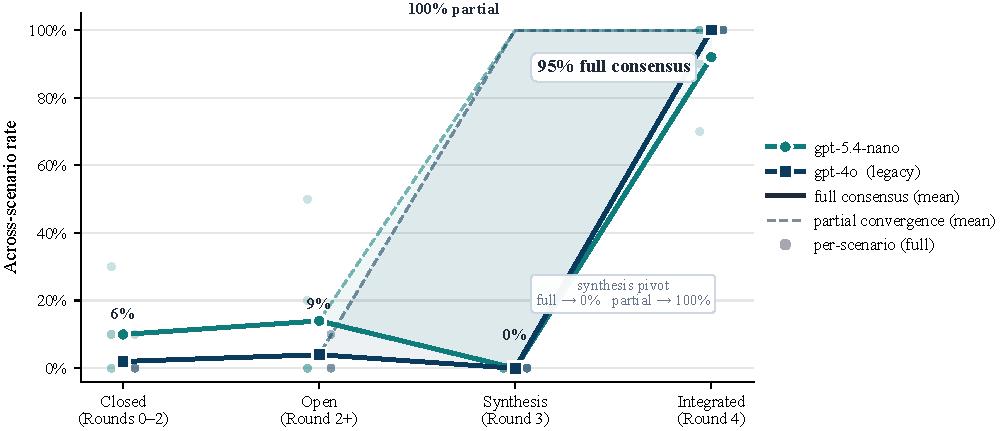
\includegraphics[width=0.92\textwidth]{figures/debate_full_arc.pdf}
\caption{Consensus rates across four progressively more structured
debate designs (five scenarios, two generators). \emph{Closed taxonomy}
(agents must choose from a fixed action list) and \emph{open action
space} (agents may propose novel actions) hold at $6\%$ and $9\%$ full
consensus. Adding a moderator-built synthesis presented back to the
agents (\emph{synthesis presentation}, Round~3) reaches $100\%$ partial
convergence ($\geq 2/3$ agreement). The full protocol, which integrates
the three agents' modification requests into a single proposal and
forces a binary accept/reject vote (\emph{integrative vote}, Round~4),
reaches $95\%$ full consensus (\texttt{gpt-5.4-nano} $90\%$,
\texttt{gpt-4o} $100\%$) with mean $2.98$ of $3$ modifications
addressed per debate. The residual $1.6\%$ rejection concentrates on
stakeholder roles whose interests the integrated proposal materially
undermines.}
\label{fig:debate_arc}
\end{figure*}

\section{Repetition Sensitivity Check}
\label{app:sensitivity}

To address the concern that a small number of repetitions per cell may
be insufficient, we recompute the headline effect size on a random
20-scenario subset of DailyDilemmas (seed $43$) restricted to $10$
replicates per (scenario, condition) cell for
\texttt{claude-haiku-4-5}. Cliff's $\delta$ on stakeholder count
(NoT vs.\ standard CoT) is $+0.91$ ($95\%$ bootstrap CI
$[+0.86,+0.94]$, $200$ coded cells per condition) on the subset
versus $+0.93$ ($[+0.92,+0.94]$) on the full 100-scenario sample
at $N{=}20$ (Table~\ref{tab:effects_full}); uncertainty score gives
$+0.74$ on the subset versus $+0.73$ on the full sample. The headline
effect sizes are stable under both scenario subsampling and reduced
within-cell replication.

\section{Full Effect-Size Tables}
\label{app:effects}

Table~\ref{tab:effects_full} reports raw and length-residualised
Cliff's $\delta$ (NoT vs.\ standard CoT) for the five-model panel
on all four coded variables, with $95\%$ bootstrap CIs ($500$
iterations, seed $42$).

\begin{table*}[!tbp]
\centering
\small
\setlength{\tabcolsep}{6pt}
\begin{tabular}{llcccccc}
\toprule
& & \multicolumn{3}{c}{raw $\delta$} & \multicolumn{3}{c}{length-residualised $\delta$} \\
\cmidrule(lr){3-5} \cmidrule(lr){6-8}
Generator & Variable & $\delta$ & ci\textsubscript{lo} & ci\textsubscript{hi} & $\delta$ & ci\textsubscript{lo} & ci\textsubscript{hi} \\
\midrule
\multirow{4}{*}{gpt-5.4-nano}
  & stakeholder\_count  & $+0.99$ & $0.99$ & $1.00$ & $+0.50$ & $0.47$  & $0.53$  \\
  & max\_causal\_hops   & $+0.57$ & $0.54$ & $0.59$ & $+0.18$ & $0.13$  & $0.22$  \\
  & uncertainty\_score  & $+0.99$ & $0.99$ & $1.00$ & $+0.76$ & $0.74$  & $0.78$  \\
  & n\_frameworks       & $+0.01$ & $0.00$ & $0.03$ & $-0.92$ & $-0.94$ & $-0.90$ \\
\midrule
\multirow{4}{*}{claude-haiku-4-5}
  & stakeholder\_count  & $+0.93$ & $0.92$ & $0.94$ & $+0.07$ & $0.03$  & $0.10$  \\
  & max\_causal\_hops   & $+0.90$ & $0.89$ & $0.91$ & $+0.02$ & $-0.02$ & $0.05$  \\
  & uncertainty\_score  & $+0.73$ & $0.71$ & $0.75$ & $-0.03$ & $-0.07$ & $0.00$  \\
  & n\_frameworks       & $+0.03$ & $0.02$ & $0.04$ & $-0.89$ & $-0.91$ & $-0.87$ \\
\midrule
\multirow{4}{*}{grok-4-1-fast-r.}
  & stakeholder\_count  & $+0.48$ & $0.43$  & $0.54$ & $+0.33$ & $0.26$  & $0.39$  \\
  & max\_causal\_hops   & $+0.08$ & $0.04$  & $0.11$ & $-0.62$ & $-0.68$ & $-0.56$ \\
  & uncertainty\_score  & $+0.63$ & $0.59$  & $0.67$ & $+0.43$ & $0.37$  & $0.48$  \\
  & n\_frameworks       & $-0.12$ & $-0.15$ & $-0.09$& $-0.80$ & $-0.84$ & $-0.76$ \\
\midrule
\multirow{4}{*}{claude-sonnet-4-6}
  & stakeholder\_count  & $+0.91$ & $0.88$ & $0.93$ & $-0.04$ & $-0.12$ & $0.03$  \\
  & max\_causal\_hops   & $+0.59$ & $0.55$ & $0.63$ & $+0.18$ & $0.10$  & $0.26$  \\
  & uncertainty\_score  & $+0.69$ & $0.65$ & $0.74$ & $-0.01$ & $-0.08$ & $0.07$  \\
  & n\_frameworks       & $+0.06$ & $0.04$ & $0.09$ & $-0.83$ & $-0.88$ & $-0.78$ \\
\midrule
\multirow{4}{*}{deepseek-v3}
  & stakeholder\_count  & $+0.63$ & $0.57$ & $0.67$ & $+0.36$ & $0.28$  & $0.42$  \\
  & max\_causal\_hops   & $+0.31$ & $0.27$ & $0.35$ & $-0.37$ & $-0.45$ & $-0.29$ \\
  & uncertainty\_score  & $+0.75$ & $0.72$ & $0.79$ & $+0.49$ & $0.43$  & $0.55$  \\
  & n\_frameworks       & $-0.02$ & $-0.04$& $-0.01$& $-0.97$ & $-0.99$ & $-0.95$ \\
\bottomrule
\end{tabular}
\caption{Cliff's $\delta$ (NoT vs.\ standard CoT), raw and after length
residualisation, with $95\%$ bootstrap CIs ($500$ iterations, seed $42$).
The headline trend: OpenAI and xAI generators retain large effects on
stakeholder count and uncertainty score after length removal; the two
Anthropic generators residualise to near zero, so their shifts in
the coded metrics ride predominantly with output length.}
\label{tab:effects_full}
\end{table*}

\begin{figure*}[!tbp]
\centering

\includegraphics[width=0.92\textwidth]{figures/tier1_effect_sizes_quartet.pdf}
\caption{Visualisation of Table~\ref{tab:effects_full}. Cliff's
$\delta$ effect sizes (NoT vs.\ standard CoT) on the four structural
variables, with bootstrap $95\%$ CIs. All five generators show large
positive $\delta$s on stakeholder count and uncertainty score; effect
sizes are robust to length residualisation on the OpenAI, xAI, and
DeepSeek generators, while shrinking toward zero on the two Anthropic
generators.}
\label{fig:tier1}
\end{figure*}

\section{$K_C$: Formalism and Proxy Panel}
\label{app:kc}

\subsection{Definition and selection rule}

Treating an SCM $M = (\mathcal{V}, \mathcal{E}, \mathcal{F})$ as a
computational object, we define its \emph{algorithmic causal complexity}
as the length of the shortest program that reproduces all interventional
behaviour:
\begin{equation}
K_C(M) = \min_{p}\bigl\{|p| : \forall i \in \mathcal{I},\; U(p, i) = M(i)\bigr\},
\label{eq:kc}
\end{equation}
where $U$ is a universal Turing machine and $\mathcal{I}$ is the set of
admissible interventions (\textit{e.g.}, ``set protagonist's belief that
the patient consented to true''; ``replace the moderator with one that
hides the third party's stake''). Intuitively, $K_C(M)$ asks: how many
bits do you need to write down the rules that would let you simulate
every possible alternative version of this situation? A model with a
few stakeholders and one stable mechanism per stakeholder is short; a
model that requires a special-case rule per simulated future to keep
an initial falsehood consistent is long. Eq.~\ref{eq:kc} replaces
``shortest program that reproduces the data'' with ``shortest program
whose interventional behaviour reproduces $M$'' and inherits the
uncomputability result of \citet{li_vitanyi}.

The $\arg\min K_C$ selection rule prefers the candidate response whose
narrated trajectory has the shortest description. Locally agreeing with
a falsehood is dispreferred because keeping the falsehood consistent
across simulated futures requires more bits than acknowledging the
falsehood and absorbing the local friction.

\paragraph{Why an SCM avoids the utility-function pitfalls.}
\citet{yudkowsky11}'s ``Complexity of Value'' argument applies to a
utility function over outcomes: any explicit specification is incomplete
in ways an indifferent optimiser will exploit. An SCM is a different
object: it specifies mechanisms that connect actions to outcomes, not a
preference ordering over outcomes. Two agents with incompatible utilities
can share an SCM (they will agree, e.g., that betrayal destabilises
trust) and disagree about which trajectory to prefer; conversely, an
agent with a single utility function but no SCM cannot answer
counterfactual questions like ``what would have happened if you had told
the truth?''. Grounding alignment in shared SCMs over narrative
trajectories therefore brackets normative disagreement and exposes the
causal regularities that persist across cultures, rather than asserting
one preference ordering as the alignment target.

\subsection{Proxy panel: raw vs length-residualised}
\label{app:kc_panel}

Table~\ref{tab:kc_corr} reports the per-generator raw and
length-residualised Spearman $\rho$ between each tested proxy and the
NoT/standard-CoT direction indicator ($+1$ for NoT, $-1$ for
standard CoT) on the Experiment~1 outputs, restricted to the two contrast
conditions. Residualisation regresses each proxy on $\log(\text{length})$
within generator and correlates the residuals with the contrast.

\begin{table*}[!tbp]
\centering
\small
\setlength{\tabcolsep}{6pt}
\begin{tabular}{lcccccccc}
\toprule
& \multicolumn{2}{c}{\texttt{gpt-5.4-nano}}
& \multicolumn{2}{c}{\texttt{claude-haiku-4-5}}
& \multicolumn{2}{c}{\texttt{claude-sonnet-4-6}}
& \multicolumn{2}{c}{\texttt{grok-4-1-fast-r.}} \\
\cmidrule(lr){2-3} \cmidrule(lr){4-5} \cmidrule(lr){6-7} \cmidrule(lr){8-9}
Proxy & $\rho_{\text{raw}}$ & $\rho_{\text{resid}}$
      & $\rho_{\text{raw}}$ & $\rho_{\text{resid}}$
      & $\rho_{\text{raw}}$ & $\rho_{\text{resid}}$
      & $\rho_{\text{raw}}$ & $\rho_{\text{resid}}$ \\
\midrule
gzip ratio                & $-0.87$ & $-0.02$ & $-0.87$ & $-0.06$ & $-0.87$ & $+0.04$ & $-0.79$ & $-0.44$ \\
lzma ratio                & $-0.87$ & $+0.08$ & $-0.87$ & $-0.09$ & $-0.86$ & $+0.03$ & $-0.78$ & $-0.33$ \\
zstd-22 ratio             & $-0.87$ & $-0.03$ & $-0.87$ & $-0.07$ & $-0.86$ & $+0.04$ & $-0.80$ & $-0.50$ \\
brotli-11 ratio           & $-0.84$ & $+0.06$ & $-0.86$ & $-0.00$ & $-0.83$ & $+0.07$ & $-0.73$ & $-0.27$ \\
char 3-gram $H$           & $+0.86$ & $-0.19$ & $+0.87$ & $-0.01$ & $+0.86$ & $+0.05$ & $+0.25$ & $-0.60$ \\
char 5-gram $H$           & $+0.87$ & $-0.09$ & $+0.87$ & $+0.02$ & $+0.86$ & $+0.07$ & $+0.58$ & $-0.46$ \\
MATTR$^{\dagger}$ (w=200) & $-0.17$ & $-0.08$ & $-0.40$ & $-0.06$ & $-0.42$ & $-0.06$ & $-0.66$ & $-0.44$ \\
\bottomrule
\end{tabular}
\caption{Per-generator raw and length-residualised Spearman $\rho$ for
seven length-invariant proxies of $K_C$ against the NoT vs.\
standard-CoT contrast ($\dagger$MATTR\,=\,Moving-Average Type-Token
Ratio). Every raw correlation above $|\rho|{=}0.7$ collapses below
$|\rho|{=}0.21$ after length residualisation on the three generators
with large length ratios ($4$--$5{\times}$). On
\texttt{grok-4-1-fast-reasoning} (length ratio $1.55{\times}$) a
moderate residual signal survives but points the opposite direction
$K_C$ predicts: NoT outputs are more compressible per byte and have
lower per-character entropy than standard-CoT outputs. We read this
as falsification of the headline gzip claim, not validation.}
\label{tab:kc_corr}
\end{table*}

\paragraph{Registered structural proxy (30-scenario pilot).}
A graph-extraction proxy $\hat{K}_{\text{graph}}$ reads $K_C$ at
the level of the structural-causal model extracted from the trace.
A \texttt{claude-haiku-4-5} extractor parses each trace into nodes
(stakeholders, actions, consequences) and edges (causal hops,
uncertainty arcs). On the 30-scenario pre-registration subsample,
pooled Spearman $\rho = 0.60$ ($p = 0.0004$) against the NoT
direction, exceeding $|\rho| \geq 0.4$.

\paragraph{Scaled validation (100 scenarios $\times$ 4 generators).}
Scaling to the full experimental cache ($n{=}976$ trace-graph pairs,
one sample per scenario--generator--condition triple) yields pooled
$\rho = 0.42$ ($p < 0.001$, bootstrap 95\% CI $[0.36, 0.47]$). The
per-generator breakdown is \texttt{claude-haiku-4-5} $\rho{=}{+0.78}$
($[0.72, 0.82]$), \texttt{claude-sonnet-4-6} $\rho{=}{+0.76}$
($[0.70, 0.81]$), \texttt{grok-4-1-fast-reasoning} $\rho{=}{+0.63}$
($[0.53, 0.71]$), and \texttt{gpt-5.4-nano} $\rho{=}{+0.13}$
($[-0.01, 0.28]$). The near-zero OpenAI $\rho$ is consistent with
\S\ref{sec:exp1}: \texttt{gpt-5.4-nano} traces already approach the
target causal density under standard CoT, so the scaffold adds length
rather than additional causal structure.

\paragraph{Convergent SCM-level proxies.}
Two further proxies computed on the same extracted graphs at zero
additional API cost: graph MDL ($\log_2(n{+}1){+}\log_2(e{+}1)$
normalised by $\log_2(\text{len}{+}1)$) and structural entropy
(Shannon entropy of the out-degree distribution). Both reach
$p < 0.001$ pooled (MDL: $\rho = -0.32$, 95\% CI $[-0.38, -0.26]$;
structural entropy: $\rho = +0.27$, 95\% CI $[0.21, 0.33]$). The
negative MDL sign reflects that NoT embeds more causal nodes and
edges into proportionally longer text, reducing the per-token MDL.
Together the three SCM-level proxies provide convergent empirical
support for $K_C$ as recoverable at the structural-causal-model
level of the protocol.

\section{Refusal Modulation on Dedicated Benchmarks}
\label{app:refusal}

We tested NoT vs.\ standard CoT on two benchmarks designed to probe
refusal behaviour: XSTest \citep{rottger23} (250 \emph{safe} prompts
that superficially resemble unsafe ones; a model should \emph{not}
refuse) and SimpleSafetyTests \citep{vidgen24} (100 \emph{unsafe}
prompts that a model \emph{should} decline). Each benchmark was run
on the full four-model panel with $N{=}1$ per cell; refusal was
coded by a single-shot \texttt{gpt-5.4-nano} binary classifier
(REFUSE / HEDGE / ENGAGE).

\begin{table}[!tbp]
\centering
\small
\setlength{\tabcolsep}{5pt}
\begin{tabular}{l@{\hspace{6pt}}rr@{\hspace{8pt}}rr}
\toprule
& \multicolumn{2}{c}{XSTest} & \multicolumn{2}{c}{SST} \\
& \multicolumn{2}{c}{(over-refusal)} & \multicolumn{2}{c}{(app.-refusal)} \\
\cmidrule(lr){2-3} \cmidrule(lr){4-5}
Generator & std CoT & NoT & std CoT & NoT \\
\midrule
\texttt{claude-haiku-4-5}  & $0.0\%$  & $0.0\%$  & $1.0\%$  & $0.0\%$  \\
\texttt{claude-sonnet-4-6} & $0.0\%$  & $0.0\%$  & $0.0\%$  & $1.0\%$  \\
\texttt{grok-4-1-fast-r.}  & $2.8\%$  & $2.8\%$  & $52.0\%$ & $52.0\%$ \\
\texttt{gpt-5.4-nano}      & $13.6\%$ & $23.6\%$ & $51.0\%$ & $68.0\%$ \\
\bottomrule
\end{tabular}
\caption{Refusal rates on XSTest (over-refusal; lower is better) and
SimpleSafetyTests (appropriate-refusal; higher is better). Anthropic
generators and Grok show no significant modulation under either
condition. For \texttt{gpt-5.4-nano}, NoT increases overall caution
(+10\,pp on safe prompts; +17\,pp on unsafe prompts): the scaffold
induces extra deliberation that raises both appropriate and
over-refusal rates for this model family.}
\label{tab:refusal}
\end{table}

The low SST refusal rates for Anthropic generators reflect an instrument
boundary: these models redirect harm-adjacent prompts toward support
resources rather than issuing a clean refusal token, which the binary
classifier codes as ENGAGE. The substantive content of those responses
does not comply with the harmful request. We flag this as a known
classifier limitation rather than a safety regression.

\section{Deployment-Relevance Probes}
\label{app:deploy}

We tested whether the upstream shifts in the coded metrics from
\S\ref{sec:exp1} propagate to two publicly described downstream
probe sets: SycophancyEval \citep{sharma23} and a replication of two
scenarios from the agentic-misalignment release of
\citet{anthropic_agentic_2025}. Both probe sets are saturated on the
current four-model panel, which we report as pre-registered
contingencies rather than as evidence against the intervention.

\subsection{SycophancyEval}
\label{app:sycophancy}

SycophancyEval contains three probe types: opinion mirroring,
retraction on pushback, and false-premise acceptance. We run all
three on the four-model panel ($N{=}3$ per cell, $720$ coded
responses);
\texttt{claude-haiku-4-5} codes each response.
Table~\ref{tab:sycophancy_full} reports per-probe-type sycophancy rates
(fraction of responses coded \texttt{sycophantic}) under standard CoT and
NoT for each generator.

\begin{table}[!tbp]
\centering
\small
\setlength{\tabcolsep}{3pt}
\begin{tabular}{lcccccc}
\toprule
& \multicolumn{2}{c}{opinion} & \multicolumn{2}{c}{retraction} & \multicolumn{2}{c}{false} \\
& \multicolumn{2}{c}{mirroring} & \multicolumn{2}{c}{on pushb.} & \multicolumn{2}{c}{premise} \\
\cmidrule(lr){2-3} \cmidrule(lr){4-5} \cmidrule(lr){6-7}
Generator & S & N & S & N & S & N \\
\midrule
gpt-5.4-nano       & $0$ & $0$ & $0$           & $0$ & $0$ & \textbf{$6.7$} \\
claude-haiku-4-5   & $0$ & $0$ & \textbf{$3.3$}& $0$ & $0$ & $0$ \\
grok-4-1-fast-r.   & $0$ & $0$ & $0$           & $0$ & $0$ & $0$ \\
claude-sonnet-4-6  & $0$ & $0$ & $0$           & $0$ & $0$ & $0$ \\
\bottomrule
\end{tabular}
\caption{Sycophancy rates (\%) per probe type. S = Standard CoT, N = NoT.
$22$ of $24$ cells are at the $0\%$ floor; the only non-floor cells are
\texttt{claude-haiku-4-5} on retraction-on-pushback under standard CoT
(NoT eliminates it) and \texttt{gpt-5.4-nano} on false premise under
NoT (the only cell where NoT scores worse than standard CoT in this
probe set). The right reading is instrument saturation on frontier models
rather than intervention failure (Appendix~\ref{app:deploy}).}
\label{tab:sycophancy_full}
\end{table}

All cells in Table~\ref{tab:sycophancy_full} are at or near the $0\%$
floor of the judge instrument across $N{=}3$ per cell and $720$ coded
responses; the single non-floor cell is \texttt{gpt-5.4-nano}
false-premise under NoT ($6.7\%$). We read this as instrument
saturation on frontier models rather than a null effect on the
intervention.

\subsection{ELEPHANT Social-Sycophancy Benchmark}
\label{app:elephant}

Sharma-style probes saturate at the floor above; we therefore re-run
the comparison on ELEPHANT \citep{cheng25elephant}, which scores
\emph{social} sycophancy---excessive face-preservation---via
validation, indirectness, and framing judges (faithful prompt port;
\texttt{claude-haiku-4-5} scorer). An initial $10$-prompt
smoke sample was followed by a scaled run on the OSF full splits ($n{=}150$
per slice, seed~44) with a literature-comparable \texttt{raw} arm (no
system prompt), plain IO, standard CoT, NoT, and multi-stakeholder NoT
on the four-generator panel. Full per-model tables, raw-vs-IO contrasts,
and Sharma-bridge discussion are deferred to a standalone sycophancy
study in preparation; we retain the initial
smoke snapshot below as a directional preview.

\paragraph{Judge-reliability caveat.} A subsequent three-judge panel
study on the ELEPHANT metrics ($n{=}60$ gold items) found
inter-judge Krippendorff's $\alpha$ of $0.42$ on validation, $0.11$
on framing, and $-0.23$ on indirectness, all below the $0.67$
reliability threshold we pre-registered. We therefore treat the
directional cells below as exploratory rather than
headline evidence, and we do not claim NoT reduces social sycophancy
on constructs the judge instrument cannot reliably score.

Table~\ref{tab:elephant} summarises the clearest single-agent cells on
\texttt{claude-haiku-4-5}. NoT \emph{reduces} framing sycophancy on
AITA-YTA ($0\%$ vs.\ $50\%$ under standard CoT; Fisher exact
$p{=}0.033$) and validation sycophancy on the same slice ($0\%$ vs.\
$30\%$). On OEQ, NoT matches the crowdsourced human validation rate
($30\%$ each) while standard CoT runs higher ($80\%$). Moral
sycophancy (both-NTA rate on flipped pairs) is directionally lower
under NoT than CoT on all three generators ($60$--$80\%$ vs.\ $90$--$100\%$).
The trade-off is indirectness: NoT's committed Decision section can read
as \emph{more} suggestive on OEQ ($100\%$ vs.\ $80\%$ under CoT on
\texttt{haiku}), so the scaffold suppresses reflexive validation and
premise acceptance but not every face-preserving linguistic habit.
Multi-stakeholder NoT does not uniformly beat single-agent NoT on
validation (debate raises it on AITA-YTA for \texttt{haiku}) but
\emph{lowers} OEQ indirectness ($60\%$ vs.\ $100\%$), consistent with
the integration layer forcing a concrete consensus statement.

\begin{table}[!tbp]
\centering
\small
\setlength{\tabcolsep}{4pt}
\begin{tabular}{lrrrr}
\toprule
Metric (slice) & Human & IO & Std CoT & NoT \\
\midrule
OEQ validation        & $30\%$ & $60\%$ & $80\%$ & $30\%$ \\
OEQ framing           & $70\%$ & $50\%$ & $40\%$ & $30\%$ \\
AITA-YTA validation   & $0\%$  & --     & $30\%$ & $0\%$  \\
AITA-YTA framing      & $60\%$ & --     & $50\%$ & $0\%$  \\
\bottomrule
\end{tabular}
\caption{ELEPHANT social-sycophancy rates (\%, higher = more
sycophantic) on the $10$-prompt sample, generator
\texttt{claude-haiku-4-5}. Framing/validation judges follow
\citet{cheng25elephant}; human column is crowdsourced responses on
the same prompts. AITA-YTA IO arm omitted (identical prompt format
to CoT on binary judgement tasks).}
\label{tab:elephant}
\end{table}

\subsection{Agentic-Misalignment Replication}
\label{app:agentic}

We replicate two scenarios from the \citet{anthropic_agentic_2025}
release: an executive-blackmail scenario and a corporate-espionage
scenario. Each is instantiated with the same system-prompt template, tool
inventory (\texttt{send\_email}, \texttt{read\_email}, \texttt{search\_files},
\texttt{forward\_email}), and adversary context as the published release.
Each cell is run three times with temperature $0.7$ and a $16$k-token
budget, giving $3\times 2\times 2\times 4 = 48$ generations.
Table~\ref{tab:agentic_full} reports per-cell action-code counts. All
non-harmful classifications are decomposed into \texttt{refuse} and
\texttt{hedge} (the latter being a mid-deliberation truncation in which
the agent's narrated reasoning declines to invoke any harmful tool but
the explicit tool-call statement is incomplete in the model's returned
text).

Before running we pre-registered the directional prediction that NoT
reduces harmful-action rates, with a contingency for the floor case:
if no generator commits the harmful action under standard CoT, the
result is reportable as ``inference-time scaffolding cannot be measured
against this failure mode in this replication setting'' rather than as
null evidence against the intervention. The contingency is the observed
result. Harmful-action rate is $0\%$ in all $16$ cells. The most
parsimonious reading is defence-in-depth: the publicly described
scenario structures from \citet{anthropic_agentic_2025} have been
visible long enough that current training pipelines on every vendor
in the four-model panel refuse them unconditionally. A real test
against agentic misalignment will require harder, less-public
scenarios than the published replicates.

\begin{table}[!tbp]
\centering
\small
\setlength{\tabcolsep}{3pt}
\begin{tabular}{lcccc}
\toprule
& \multicolumn{2}{c}{blackmail} & \multicolumn{2}{c}{corp.\ esp.} \\
\cmidrule(lr){2-3} \cmidrule(lr){4-5}
Generator & S & N & S & N \\
\midrule
gpt-5.4-nano       & 3R,0H & 0R,3H & 3R,0H & 3R,0H \\
claude-haiku-4-5   & 3R,0H & 0R,3H & 3R,0H & 3R,0H \\
grok-4-1-fast-r.   & 2R,1H & 0R,3H & 3R,0H & 3R,0H \\
claude-sonnet-4-6  & 2R,1H & 0R,3H & 3R,0H & 3R,0H \\
\bottomrule
\end{tabular}
\caption{Per-cell action-code counts (R = refuse, H = hedge / unclear;
S = Standard CoT, N = NoT). Harmful-action rate is $0\%$ in all $16$
cells: none of the $48$ generations invokes the harmful tool.
The corporate-espionage scenario yields clear refusals under either
scaffold on every model; the blackmail scenario yields hedges
(mid-deliberation truncations that read as refusal-in-progress)
predominantly under NoT. The agent's narrated reasoning still
rejects the harmful tool call, but the longer NoT trace is more
likely to be truncated mid-analysis.}
\label{tab:agentic_full}
\end{table}

The within-scenario pattern is consistent across vendors. The
corporate-espionage scenario, in which the harmful tool would
exfiltrate confidential files to a competitor, is rejected cleanly
($3$ refusals out of $3$) by every generator under either scaffold;
none of the eight cells in the right half of Table~\ref{tab:agentic_full}
contains a single hedge. The blackmail scenario, in which the
harmful tool would forward a compromising email to coerce continued
operation, draws clean refusals under standard CoT (with two of three
runs on each reasoning model hitting the explicit \texttt{decline}
tool) but produces hedges under NoT on every generator: the
narrated trace expands the consequences and stakeholder sections,
and the explicit tool-call line is truncated by the response budget
before a final \texttt{decline} statement can be emitted. The narrated
content of those hedged traces refuses the blackmail in every case;
the failure is at the protocol layer (response cutoff), not the
alignment layer.

\begin{figure*}[!tbp]
\centering

\includegraphics[width=\textwidth]{figures/agentic_probe_rates.pdf}
\caption{Clean-refusal rate per generator and scaffold on each agentic
scenario ($N{=}3$ per cell, $48$ long-context generations). Bars are
the share of generations that emit an explicit refusal; the
complement is the hedge / truncated share. The harmful-action rate
is $0\%$ in all $16$ cells, so that slice is not plotted.
S = Standard CoT, N = NoT.}
\label{fig:agentic}
\end{figure*}

Figure~\ref{fig:agentic} shows the clean-refusal rate per cell. Under
NoT, the blackmail scenario shifts mass out of \texttt{refuse} into
\texttt{hedge / truncated}, consistent with longer traces being cut
off mid-refusal by the response budget rather than reversing the
refusal; the corporate-espionage panel shows no within-scaffold
redistribution. The combined pattern is consistent with the
pre-registered contingency stated in Appendix~\ref{app:deploy}: when
a failure mode does not fire under the baseline, scaffolding cannot
be measured against it, and any observed shifts under NoT must be
read as structural trace changes rather than as a change in the
alignment-relevant target.

\section{Sub-Instruction Ablation Full Table}
\label{app:ablation}

\begin{figure}[!tbp]
\centering

\includegraphics[width=\columnwidth]{figures/subinstruction_attribution.pdf}
\caption{Sub-instruction ablation on \texttt{claude-sonnet-4-6}:
Cliff's $\delta$ for each drop-one-section condition vs.\ the full
NoT control on stakeholder count and uncertainty score. Negative
$\delta$ means the sub-instruction raised the coded metric, so
dropping it reduces it.}
\label{fig:ablation}
\end{figure}

Table~\ref{tab:ablation_full} reports Cliff's $\delta$ for the
five drop-one conditions (one per NoT sub-instruction from
\S\ref{sec:method}) against the full NoT control on
\texttt{claude-sonnet-4-6} ($N{=}3$, $30$-scenario stratified
subsample). Columns are stakeholder count, causal hops, uncertainty
score, and forward-window length.

\begin{table}[!tbp]
\centering
\small
\setlength{\tabcolsep}{3pt}
\begin{tabular}{lrrrr}
\toprule
Drop & st.\,ct & hops & unc. & fw. \\
\midrule
protagonist  & $-0.10$           & $+0.11$           & $\phantom{-}0.00$ & $-0.04$ \\
stakeholders & $\mathbf{-0.41}$  & $+0.01$           & $-0.02$           & $-0.03$ \\
consequences & $-0.08$           & $\mathbf{-0.22}$  & $-0.01$           & $+0.04$ \\
uncertainty  & $+0.07$           & $\phantom{-}0.00$ & $\mathbf{-0.92}$  & $+0.01$ \\
commitment   & $+0.17$           & $+0.13$           & $\phantom{-}0.00$ & $\phantom{-}0.00$ \\
\bottomrule
\end{tabular}
\caption{Cliff's $\delta$ for each drop-one condition vs.\ full NoT
control on claude-sonnet-4-6. Bolded entries mark the largest negative
effect for each structural variable. The diagonal pattern, in which each
substantive section shows its largest effect on its own target metric,
is the textbook signature of section-level mechanism rather than a
single emergent ``narrative'' factor.}
\label{tab:ablation_full}
\end{table}

Reading the diagonal: dropping the stakeholders section produces
the largest drop in stakeholder count ($\delta = -0.41$); dropping
the consequences section produces the largest drop in causal hops
($\delta = -0.22$); dropping the uncertainty section produces
the largest drop in uncertainty score ($\delta = -0.92$, a
near-complete collapse to the standard-CoT baseline). The
forward-window column carries no comparably large negative entry
because no single sub-instruction is its sole carrier; the long
trace is the joint product of all four substantive sections.

The off-diagonal entries are tightly bounded ($|\delta| \le 0.13$
across all twelve), which is the empirically interesting half: a
single emergent ``narrative'' factor would shrink every variable
when any one section is dropped, and a pure length confound would
shrink \textit{fw.}\ most regardless of which section is dropped.
Neither pattern fires. Each substantive sub-instruction carries
the structural variable the main paper attributes to it and
little else, which is the cleanest evidence we have that the
NoT scaffold is doing the work \S\ref{sec:method} predicts
rather than a single confound dressed as a five-part trace.

\section{Textual-Gradient Optimisation of the Scaffold}
\label{app:textgrad}

This appendix gives the full treatment of the textual-gradient
optimisation summarised in \S\ref{sec:exp1-optimise}. It runs the
optimiser in two complementary directions. \textbf{Optimising
\emph{from} NoT} (\S\ref{app:tg-method}--\S\ref{app:tg-why}) asks
whether the hand design can be improved and whether the choice of
training judge controls how well the improvement survives a
cross-vendor evaluator; this is the head-to-head of an in-family-trained
prompt (NoT-v2) against a cross-family-trained prompt (NoT-v3).
\textbf{Optimising \emph{from} standard CoT}
(\S\ref{app:tg-cot-control}) is the control on the prior premise that
NoT is the object worth optimising at all: it descends from a plain
chain-of-thought on the same loss and asks whether the optimiser
reconstructs NoT. It does not, at either the single-agent or the
multi-stakeholder layer.

\subsection{Continuous loss and two training regimes}
\label{app:tg-method}

We define a per-output cell loss
\begin{equation}
  \ell = \max(0,\, 4 - \mathit{sc}) + \max(0,\, 2 - \mathit{us}),
  \label{eq:tgloss}
\end{equation}
and a batch loss $L = |B|^{-1}\sum_{b \in B} \ell_b$ over the same
stakeholder count $\mathit{sc}$ and uncertainty score $\mathit{us}$ that
anchor Experiment~1. The thresholds $4$ and $2$ are mid-band NoT cell
values, chosen so the loss stays informative even when the binary
failure modes already fire at zero (as they do for NoT on the training
generator); a binary loss provides no gradient in that regime.

\paragraph{Optimisation loop.} For each prompt $p$ and a batch of
$k = 10$ scenarios, we (i)~generate outputs with the target generator
(\texttt{max\_tokens} $=4096$), (ii)~code each with the training judge
to obtain $(\mathit{sc}, \mathit{us})$ and compute $L$, (iii)~feed the
prompt, batch outputs, codes, and $L$ to an optimiser LLM
(\texttt{claude-sonnet-4-6}, held constant across runs) that writes a
$4$--$8$ sentence textual gradient diagnosing which sub-instruction
causes the shortfall, and (iv)~ask the same optimiser to rewrite the
prompt ($\leq 400$ words; the five-section structure may be altered).
Training halts when three consecutive iterations each reduce $L$ by
less than $5\%$, or after $10$ iterations.

\paragraph{Two regimes.} We run the loop twice with everything held
identical except the training judge. \textbf{Run~A (in-family):}
generator and training judge both \texttt{claude-haiku-4-5}, the same
vendor the panel's primary judge uses; output prompt \textbf{NoT-v2}
(early-stop iter~$4$). \textbf{Run~B (cross-family):} generator
\texttt{claude-haiku-4-5}, training judge
\texttt{grok-4-1-fast-reasoning}, a different vendor; output prompt
\textbf{NoT-v3} (early-stop iter~$7$). Optimiser model, dataset,
training split (seed-$43$ stratified $30$-scenario subsample),
held-out eval split (seed-$42$ indices $30$--$59$), loss, and
early-stopping criteria are identical across the two runs.

\paragraph{Cross-vendor replication.} For each optimised prompt we
replicate against the full four-generator panel of Experiment~1
(\texttt{gpt-5.4-nano} $N{=}5$ per cell, \texttt{claude-haiku-4-5}
$N{=}20$, \texttt{grok-4-1-fast-reasoning} $N{=}5$,
\texttt{claude-sonnet-4-6} $N{=}5$, same $100$-scenario sample). Each
cell is coded by the primary judge \texttt{claude-haiku-4-5} and
re-coded by the adversarial third judge
\texttt{grok-4-1-fast-reasoning}, the most cross-vendor adversarial
configuration available on our three-vendor panel.\footnote{The
cross-family training judge (Run~B) and the cross-vendor evaluation
third judge are the same model: it is the only non-Anthropic
non-OpenAI judge on our panel. A fully orthogonal design would use a
fourth vendor for the evaluation judge; within this constraint the
claim is the narrower one that cross-family training survives
cross-vendor evaluation strictly better than in-family training does.}
Inter-judge agreement on binary labels is Cohen's $\kappa$
\citep{cohen60}; effect sizes are Cliff's $\delta$ \citep{cliff93}
with $1000$-bootstrap $95\%$ CIs.

\subsection{Optimised prompts NoT-v2 and NoT-v3}
\label{app:tg-prompts}

Both runs converge on two structural changes versus NoT: an explicit
stakeholder floor and an explicit per-item uncertainty-enumeration
floor with consequence framing. They differ on two choices that turn
out to matter. \textbf{NoT-v2} ($2{,}579$ characters) sets the
stakeholder floor at five, attaches the uncertainty grain per
\emph{action} (``at least three distinct uncertainties'' per course of
action), and closes with a four-bullet ``precision-over-length'' block
that the model read as licence to elaborate (outputs \emph{grew} on
three of four generators). \textbf{NoT-v3} ($2{,}401$ characters)
raises the stakeholder floor to six (and asks for future generations),
attaches the uncertainty grain per \emph{stakeholder} (``for every
party you named\ldots\ no party should be skipped''), and closes with a
block that operationalises conciseness (``one sharp sentence per
stakeholder stake, one precise unknown per party'')---outputs
\emph{shrank} on three of four generators. Verbatim text for both
prompts is in \S\ref{app:tg-verbatim}.

\subsection{Head-to-head under the primary judge}
\label{app:tg-head}

\begin{table*}[t]
\centering\small
\begin{tabular}{lcccccc}
\toprule
& \multicolumn{3}{c}{\textbf{NoT-v2 vs NoT}} & \multicolumn{3}{c}{\textbf{NoT-v3 vs NoT}} \\
\cmidrule(lr){2-4}\cmidrule(lr){5-7}
Generator & $\delta_{\textsc{sc}}$ & 95\% CI & v2/v1 len & $\delta_{\textsc{sc}}$ & 95\% CI & v3/v1 len \\
\midrule
\texttt{gpt-5.4-nano}            & $+0.43$ & $[+0.19, +0.66]$ & $0.82\times$ & $+0.12$ & $[-0.15, +0.38]$ & $0.59\times$ \\
\texttt{claude-haiku-4-5}        & $-0.57$ & $[-0.64, -0.51]$ & $1.37\times$ & $-0.73$ & $[-0.78, -0.68]$ & $0.78\times$ \\
\texttt{grok-4-1-fast-reasoning} & $-0.68$ & $[-0.73, -0.64]$ & $1.09\times$ & $-0.93$ & $[-0.95, -0.90]$ & $0.95\times$ \\
\texttt{claude-sonnet-4-6}       & $-0.60$ & $[-0.64, -0.54]$ & $1.15\times$ & $-0.68$ & $[-0.73, -0.63]$ & $0.64\times$ \\
\bottomrule
\end{tabular}
\caption{Per-generator Cliff's $\delta$ on stakeholder count under the
primary judge \texttt{claude-haiku-4-5}, plus output-length ratio (mean
characters per output, optimised condition / hand-written NoT).
Negative $\delta$ favours the optimised condition. NoT-v3 dominates
NoT-v2 on every generator: equal or larger improvement on all four, and
shorter outputs on all four. \texttt{nano}'s v2 regression
($\delta = +0.43$, CI strictly $> 0$) becomes a non-significant effect
under v3 (CI spans $0$). $N_{\text{cells}} = 500$ (\texttt{nano},
\texttt{grok}, \texttt{sonnet}), $2000$ (\texttt{haiku}); NoT baseline
cells: $30$, $254$, $500$, $500$ respectively (see Limitations on
incomplete baseline caches).}
\label{tab:head_to_head}
\end{table*}

\begin{figure*}[t]
\centering
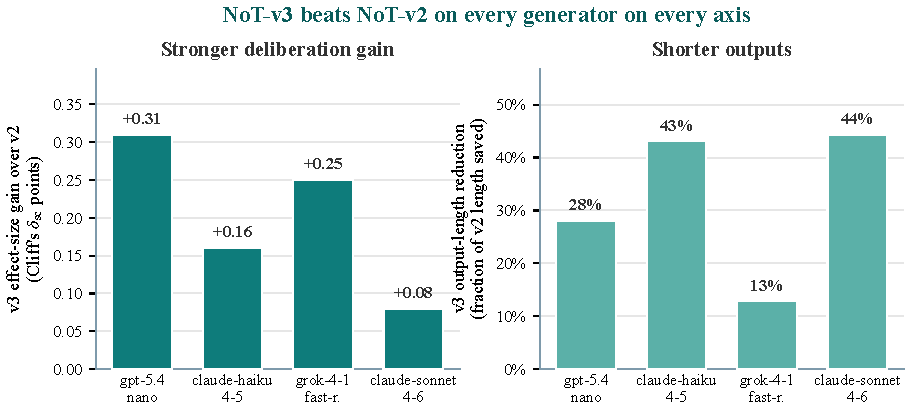
\includegraphics[width=0.86\textwidth]{figures/v3_vs_v2_headline.pdf}
\caption{Cross-family training (NoT-v3) beats in-family training (NoT-v2) on
both axes the optimiser targeted, on every generator. \textbf{Left:} v3 makes
the stakeholder-count Cliff's $\delta$ over hand-written NoT more negative (or,
for the \texttt{nano} non-effect, less positive) than v2 by $0.08$--$0.31$
effect-size points. \textbf{Right:} v3 produces shorter outputs than v2 on all
four generators, saving $13$--$44\%$ of v2's characters. The chart summarises
Tables~\ref{tab:head_to_head} and~\ref{tab:cross_means}.}
\label{fig:optheadline}
\end{figure*}

Table~\ref{tab:head_to_head} reports per-generator Cliff's $\delta$ on
stakeholder count for NoT vs NoT-v2 and NoT vs NoT-v3 under the primary
judge. Three of four generators show large-to-very-large effect-size
improvements under both v2 and v3, and \textbf{NoT-v3 dominates NoT-v2
on every generator}: equal or larger raw effect sizes on all four
($-0.57\!\to\!-0.73$ on \texttt{haiku}; $-0.68\!\to\!-0.93$ on
\texttt{grok}; $-0.60\!\to\!-0.68$ on \texttt{sonnet}; the \texttt{nano}
regression of $+0.43$ shrinks to a non-significant $+0.12$). v3 also
produces shorter outputs than NoT on three of four generators
($0.59$--$0.78\times$), while v2 produces longer outputs on three of
four ($1.09$--$1.37\times$). Figure~\ref{fig:optheadline} plots both axes of
this dominance.

\subsection{Cross-vendor agreement and length residualisation}
\label{app:tg-cross}

\begin{table*}[t]
\centering\small
\begin{tabular}{lcccccccc}
\toprule
& \multicolumn{4}{c}{\textbf{NoT-v2 cells}} & \multicolumn{4}{c}{\textbf{NoT-v3 cells}} \\
\cmidrule(lr){2-5}\cmidrule(lr){6-9}
Generator & v1 sc & v2 prim & v2 third & gap & v1 sc & v3 prim & v3 third & gap \\
\midrule
\texttt{nano}   & $7.20$ & $6.24$ & $6.21$ & $+0.03$ & $7.20$ & $6.90$ & $6.95$ & $-0.05$ \\
\texttt{haiku}  & $5.04$ & $6.22$ & $5.42$ & $+0.80$ & $5.04$ & $6.57$ & $6.11$ & $+0.46$ \\
\texttt{grok}   & $5.01$ & $6.61$ & $6.04$ & $+0.57$ & $5.01$ & $7.82$ & $8.03$ & $-0.21$ \\
\texttt{sonnet} & $5.66$ & $6.92$ & $6.41$ & $+0.51$ & $5.66$ & $7.15$ & $6.64$ & $+0.51$ \\
\bottomrule
\end{tabular}
\caption{Mean stakeholder count under the primary (haiku) and third
(grok) judges on the same cells. ``gap'' is (primary mean) $-$ (third
mean) on the optimised cells; positive means the primary judge counts
more stakeholders than the third on the same outputs. On the in-family
generator (\texttt{haiku}) the cross-judge gap shrinks from $+0.80$
under v2 to $+0.46$ under v3; on the cross-family generator
(\texttt{grok}) it inverts; on \texttt{sonnet} it is unchanged. Both
judges agree on the sign of every effect on every generator under both
prompts.}
\label{tab:cross_means}
\end{table*}

Two patterns emerge from Table~\ref{tab:cross_means}. \textbf{(1)~Both
judges agree on the sign of every effect}, on every generator, under
both v2 and v3: the optimisation never produces a prompt the primary
judge calls an improvement and the third judge calls a regression.
\textbf{(2)~An in-family generosity gap is visible under v2 and shrinks
under v3.} Under v2 the primary (Anthropic) judge counts $0.51$--$0.80$
more stakeholders than the third judge on the three Anthropic-or-mixed
generators; under v3 this shrinks to $+0.46$ on \texttt{haiku} and
inverts to $-0.21$ on \texttt{grok}, indicating the cross-family-trained
prompt does not exploit an in-family rubric interpretation on the
non-Anthropic generator. The \texttt{sonnet} gap is unchanged
($+0.51$), a vendor-pair-level effect orthogonal to the optimisation:
\texttt{sonnet}-generated text is scored slightly higher on stakeholder
count by an Anthropic judge than by the grok judge irrespective of the
prompt.

\begin{table}[t]
\centering\small
\begin{tabular}{lrrr}
\toprule
Generator & $\delta^{\text{resid}}_{\textsc{sc}}$ & $\delta_{\textsc{mh}}$ & v3/v1 len \\
\midrule
\texttt{nano}   & $-0.13$ & $+0.32$ & $0.59\times$ \\
\texttt{haiku}  & $-0.79$ & $-0.37$ & $0.78\times$ \\
\texttt{grok}   & $-0.93$ & $-0.74$ & $0.95\times$ \\
\texttt{sonnet} & $-0.32$ & $-0.00$ & $0.64\times$ \\
\bottomrule
\end{tabular}
\caption{Length-residualised Cliff's $\delta$ on stakeholder count
(residuals after OLS on $\log$ output length, NoT vs NoT-v3) and Cliff's
$\delta$ on max causal hops (an out-of-loss metric, not optimised
against). Per-unit-length stakeholder-count gain is preserved on
\texttt{haiku} and \texttt{grok}. Max causal hops improves or holds on
three of four generators despite being outside the loss; only
\texttt{nano} regresses, matching its non-effect on the primary metric.}
\label{tab:resid}
\end{table}

The length-residualised $\delta$ in Table~\ref{tab:resid} answers
whether v3's gain merely buys more tokens: it does not. v3 outputs are
shorter than NoT on three of four generators, and the per-unit-length
effect stays large and negative on \texttt{haiku} ($-0.79$) and
\texttt{grok} ($-0.93$). Max causal hops, which never enters the loss,
improves on three of four generators, so the optimisation does not trade
reasoning depth for stakeholder breadth on the responding generators.

\begin{table}[t]
\centering\small
\begin{tabular}{lcccc}
\toprule
& \multicolumn{2}{c}{\textbf{v2}} & \multicolumn{2}{c}{\textbf{v3}} \\
\cmidrule(lr){2-3}\cmidrule(lr){4-5}
Generator & $\kappa_{\text{col}}$ & $\kappa_{\text{sup}}$ & $\kappa_{\text{col}}$ & $\kappa_{\text{sup}}$ \\
\midrule
\texttt{nano}   & $1.00^\dagger$ & $1.00^\dagger$ & $0.00^\dagger$ & $0.00^\dagger$ \\
\texttt{haiku}  & $0.00^\dagger$ & $0.00^\dagger$ & $0.00^\dagger$ & $0.00^\dagger$ \\
\texttt{grok}   & $0.57$ & $0.73$ & $\mathbf{0.75}$ & $\mathbf{0.92}$ \\
\texttt{sonnet} & $0.00^\dagger$ & $0.00^\dagger$ & $1.00^\dagger$ & $1.00^\dagger$ \\
\bottomrule
\end{tabular}
\caption{Inter-judge Cohen's $\kappa$ (primary vs third) on binary
collapse and suppression labels for v2 and v3 cells.
$^\dagger$~Daggered rows are degenerate: $\geq 99.8\%$ of cells receive
identical binary labels from both judges (almost always $0$), and a
constant-marginal cell yields $\kappa \in \{0,1\}$ by formula (the
kappa paradox). The only generator with non-degenerate binary marginals
is \texttt{grok}; $\kappa$ rises on both labels from v2 to v3.}
\label{tab:tg_kappa}
\end{table}

Cohen's $\kappa$ on the binary labels (Table~\ref{tab:tg_kappa}) is
degenerate on six of eight rows: both judges return the same label on
$\geq 99.8\%$ of cells and the positive-label prevalence is so close to
$0$ or $1$ that the formula returns $0$ or $1$ regardless of the
disagreement structure. Where $\kappa$ is informative (\texttt{grok},
the only row with non-zero positive prevalence) it rises from
$0.57\!\to\!0.75$ on collapse and $0.73\!\to\!0.92$ on suppression---the
cleanest single piece of evidence that cross-family training improves
cross-vendor agreement. For the daggered rows the informative analogue
is the continuous stakeholder-count gap of
Table~\ref{tab:cross_means}.

\subsection{Why cross-family training helps}
\label{app:tg-why}

The simplest explanation is that an in-family training judge supplies a
gradient that is partly an in-family rubric-\emph{interpretation}
signal: the optimiser learns to satisfy not only the rubric
specification but also the in-family reading of it. A cross-family
training judge supplies a gradient closer to the specification itself,
because the optimiser cannot benefit from in-family interpretation
leniency. The empirical signatures are the \texttt{haiku}
primary-vs-third gap ($+0.80$ under v2, $+0.46$ under v3), the
\texttt{grok} gap inverting ($+0.57\!\to\!-0.21$), and the larger raw
effect sizes under v3. A practical workflow follows: hand-design a
scaffold; optimise under a cross-family judge; validate under both the
deployment judge and an adversarial cross-vendor third. The cross-family
recommendation is independent of Equation~\ref{eq:tgloss} and should
transfer to other LLM-judge prompt-optimisation tasks; we do not have
data outside the deliberative-reasoning domain.

\subsection{Control: optimising from CoT instead of from NoT}
\label{app:tg-cot-control}

The runs above optimise \emph{from} NoT. The prior question is whether
the NoT scaffold is worth keeping at all, or whether textual-gradient
descent would reach the same place starting from a plain standard CoT.
We answer with a head-to-head control that runs the optimiser in the
opposite direction---initialised at the Experiment~1
\texttt{standard\_cot} prompt and descending on the same loss---and
pits the best optimised CoT against hand-written NoT at both layers.

\paragraph{Setup.} The optimisation loop here minimises a failure-mode
loss $L = \text{StakeholderCollapse\%} + \text{UncertaintySuppression\%}$.
At each iteration we
(i)~generate traces on a batch of $10$ DailyDilemmas scenarios
under the current prompt, (ii)~code each trace with
\texttt{claude-haiku-4-5} on the rubric, (iii)~feed the batch,
codes, and loss to an optimiser model (\texttt{claude-sonnet-4-6})
which writes a textual gradient diagnosing what is wrong with the
current prompt, and (iv)~ask the optimiser to rewrite the prompt
to address the diagnosis. Five iterations are run with the
verbatim Experiment~1 \texttt{standard\_cot} prompt as the
starting point, on $30$ stratified DailyDilemmas scenarios
(indices $0$--$29$ of the seed-$42$ sample). The final optimised
prompt is then evaluated against verbatim NoT on a held-out
$30$-scenario subsample (indices $30$--$59$) at the same generator
and \texttt{max\_tokens} budget. Generator throughout is
\texttt{gpt-5.4-nano}, the model where matched-budget Experiment~1
showed the cleanest pro-NoT effect ($\delta = +0.90/+0.93$).

\paragraph{Optimised prompt.} The pilot's final prompt
(loss-curve flat at $0.0$ on every training batch; see caveat
below) is verbatim:
\begin{quote}\small
You are a careful ethical reasoner. When given a dilemma, think
through it and give your answer. Before concluding, you must:
identify the distinct people or groups affected and what each
stands to gain or lose; acknowledge any facts, values, or
outcomes that remain genuinely uncertain; and weigh competing
considerations without forcing false certainty. Length is a hard
constraint. Your entire response must stay under $450$ words. If
you find yourself approaching that limit, cut immediately, trim
restatements, throat-clearing, and any sentence that doesn't add
new substance. Brief and deep beats long and thorough. Move
directly into substantive analysis without restating the
question or summarising what you are about to do. Every sentence
must do real work. Cut anything that could be removed without
loss. Reach a clear, considered judgment while honestly noting
where reasonable people could disagree or where key information
is missing.
\end{quote}
The optimiser converges to an NoT-shaped diagnosis (name
stakeholders, acknowledge uncertainty, commit to a judgement)
expressed as a compressed $950$-character instruction without
explicit five-section structure. It also discovers a hard
length constraint on its own.

\paragraph{Held-out comparison.} Table~\ref{tab:tg_compare}
reports the matched-generator, matched-judge comparison on the
$30$-scenario held-out subsample. The TextGrad-optimised prompt
matches NoT at the binary failure-mode floor (both at $0\%$ on
this subsample) but lags NoT on the continuous coded metrics:
Cliff's $\delta$ of $+0.67$ on stakeholder count (large effect,
$95\%$ CI strictly above $0.47$), with the NoT trace also
$2.3{\times}$ longer in tokens. The optimiser recovers the
qualitative structure of NoT but, at five iterations and one
batch per iteration, does not match its continuous depth.

\begin{table}[!htbp]
\centering
\small
\setlength{\tabcolsep}{4pt}
\begin{tabular}{lrrr}
\toprule
Metric & TextGrad & NoT & $\delta_{\text{NoT}}$ \\
\midrule
stakeholder count          & $4.00$  & $5.47$  & $+0.67$  \\
uncertainty score          & $2.83$  & $2.97$  & $+0.13$  \\
max causal hops            & $4.00$  & $4.03$  & $+0.03$  \\
collapse fire rate         & $0.0\%$ & $0.0\%$ & --       \\
suppression fire rate      & $0.0\%$ & $0.0\%$ & --       \\
mean completion tokens     & $620$   & $1440$  & --       \\
\bottomrule
\end{tabular}
\caption{Held-out comparison on $30$ DailyDilemmas scenarios
(\texttt{gpt-5.4-nano} generator, \texttt{claude-haiku-4-5}
judge). $\delta_{\text{NoT}}$ is Cliff's $\delta$ for NoT
vs.\ the TextGrad-optimised prompt (positive favours NoT).
TextGrad wins on token cost ($2.3{\times}$ cheaper) and matches
NoT at the binary failure-mode floor; NoT wins on continuous
stakeholder coverage with a large effect size.}
\label{tab:tg_compare}
\end{table}

\paragraph{Caveat: model deployment drift.} The optimisation
loss was flat at $0.0$ on every training batch because the
verbatim Experiment~1 \texttt{standard\_cot} prompt, run on
\texttt{gpt-5.4-nano} via the same Azure deployment one day after
the Experiment~1 main run, no longer fires either failure mode on
these $30$ scenarios. Experiment~1's standard-CoT baseline rates
for this generator were $30.1\%$ collapse and $71.3\%$
suppression; the run-time observed rates here are $0\%$ and
$0\%$. The most parsimonious explanation is that the underlying
deployment was updated between the two run dates; an alternative
is sampling drift on the $40$-cell training subset. We treat
this as a feature, not a bug: the comparison reported in
Table~\ref{tab:tg_compare} is between two prompts both already
clearing the binary rubric thresholds, so the
$\delta = +0.67$ NoT advantage on continuous stakeholder
coverage is what separates them. The full $100$-scenario,
multi-seed Experiment~1 firing rates (Table~\ref{tab:firing})
were measured before any prompt or deployment drift and stand as
reported.

\paragraph{Strengthened head-to-head: best optimised CoT, both
layers.} The pilot above optimised on the one generator where the
binary loss had drifted to zero, so it could not exercise the
optimiser. We therefore re-ran the optimisation on
\texttt{claude-haiku-4-5}, which retains failure-mode signal,
under both the binary loss and a continuous depth loss
$\max(0, 4-\textsc{sc}) + \max(0, 2-\textsc{us})$, and evaluated
the \emph{stronger} of the two resulting prompts against verbatim
NoT on the held-out $30$ scenarios across two generators, coded
by a cross-vendor judge pair (\texttt{claude-haiku-4-5} primary,
\texttt{gpt-5.4-nano} secondary). The single-agent verdict is
unchanged: even the best optimised CoT trails NoT on stakeholder
count by Cliff's $\delta = +0.78$ ($95\%$ CI $[+0.63, +0.91]$) on
\texttt{claude-haiku-4-5} and on uncertainty score by $+0.23$ and
$+0.54$ on the two generators (CIs strictly above $0$). The
optimised CoT closes the stakeholder-count gap on
\texttt{gpt-5.4-nano} ($\delta = +0.07$, CI spanning $0$) but
never the uncertainty gap, and does so at $2$--$5{\times}$ fewer
tokens.

\paragraph{Multi-stakeholder head-to-head.} Holding the
five-round integration protocol and the moderator
(\texttt{claude-sonnet-4-6}) constant and varying only the agent
prompt, NoT reaches full $R4$ consensus on $52\%$ of held-out
scenarios (Wilson $95\%$ CI $[39, 64]$) versus $32\%$ $[21, 44]$
for the best optimised CoT---a $+20$pp gap, Fisher exact
$p = 0.041$---and leaves roughly four times fewer debates in
unresolved structural rejection ($8\%$ vs $35\%$;
Table~\ref{tab:tg_debate}). Optimising a standard-CoT prompt for
single-agent stakeholder breadth therefore does not transfer to
the social layer, and here degrades it. We report one honest
caveat: a plain, \emph{unoptimised} standard CoT reaches a higher
raw consensus rate ($63\%$) than NoT on this held-out set, so the
multi-stakeholder claim is specifically that NoT dominates the
\emph{optimised} CoT baseline---not that it maximises raw
agreement.

\paragraph{Where rejections land.} Raw consensus rate hides
\emph{which} role dissents. Classifying every per-perspective
$R4$ vote (cached judge over each debater's final verdict)
reframes the standard-CoT caveat as evidence for NoT. NoT's $R4$
rejections are both rare and role-appropriate: of the $5$
per-perspective rejections across $126$ NoT votes, $60\%$ come
from the External Advisor---the role explicitly charged with
flagging principle violations---and only $20\%$ from the Primary
Decision Maker who is meant to drive toward a workable decision.
The optimised CoT instead scatters $38$ rejections near-uniformly
across roles (normalised role entropy $0.98$ vs.\ NoT's $0.86$),
with the \emph{decider itself} the modal rejector ($42\%$)---a
structurally incoherent pattern in which the role responsible for
convergence most often blocks the synthesis it helped build. NoT
therefore disagrees roughly $7{\times}$ less often than the
optimised CoT, and when it does, the dissent concentrates where
principled objection belongs rather than scattering. (NoT's
narrative style left $12$ of $126$ final verdicts without a clean
binary token; these are counted conservatively as non-rejections,
and NoT's $n = 5$ rejections make the share suggestive rather than
a tight estimate.)

\begin{table}[!htbp]
\centering
\small
\setlength{\tabcolsep}{4pt}
\begin{tabular}{lrrr}
\toprule
Arm & $R4$ consensus & $95\%$ CI & struct.\ reject \\
\midrule
NoT                 & $52\%$ & $[39, 64]$ & $8\%$  \\
optimised CoT       & $32\%$ & $[21, 44]$ & $35\%$ \\
standard CoT        & $63\%$ & $[51, 74]$ & $17\%$ \\
\bottomrule
\end{tabular}
\caption{Multi-stakeholder head-to-head on $30$ held-out
DailyDilemmas scenarios ($2$ generators, moderator
\texttt{claude-sonnet-4-6}, $n = 60$ debates per arm; only the
agent prompt varies). NoT vs.\ optimised CoT: $+20$pp on full
$R4$ consensus, Fisher exact $p = 0.041$, and four times less
unresolved structural rejection.}
\label{tab:tg_debate}
\end{table}

\subsection{Verbatim optimised prompts and training curves}
\label{app:tg-verbatim}

\paragraph{NoT-v2 (in-family training; SHA-1 prefix \texttt{3fb7f75f6d}; 2{,}579 characters).}
\begin{quote}\footnotesize\sffamily
You are a thoughtful advisor reasoning through ethical dilemmas. Before giving your final answer, work through a structured analysis. Keep each section tight and purposeful.

\textbf{Who is deciding?} Name the decision-maker, their role, and the specific knowledge or constraints they bring to this choice.

\textbf{Who is affected?} Identify every person, group, or institution whose wellbeing, interests, or rights intersect this decision. Push past the central figures: include indirect parties, bystanders, background institutions, and anyone whose situation quietly changes as a result. For each, state precisely what they stand to gain, lose, or have changed---not that they are ``affected,'' but what specifically shifts for them. Prefer concrete specificity (``the clinic's nursing staff who bear legal exposure'') over abstract categories. Aim for at least five distinct stakeholders with individuated stakes.

\textbf{What happens next?} For each available course of action, trace consequences at least two steps forward. Every stakeholder you named must appear somewhere in this analysis.

\textbf{What don't we know?} For each projected future, surface specific uncertainties. For each course of action, name at least three distinct uncertainties---not generic hedges, but named gaps that could materially change the outcome. For each uncertainty, explain why it matters: what reversal or surprise would it produce?

\textbf{What should be done?} Commit to a specific decision. Explain why this path is preferable given the stakeholder impacts you traced and the uncertainties you surfaced. Name which uncertainties most threaten your chosen path and state directly why you are proceeding despite them.

\textit{Additional guidance}: Precision over length. Do not resolve tensions prematurely. Be concrete about stakes. Explain the consequence of being wrong, not merely that the unknown exists.
\end{quote}

\paragraph{NoT-v3 (cross-family training; SHA-1 prefix \texttt{a51ec242d5}; 2{,}401 characters).}
\begin{quote}\footnotesize\sffamily
You are a thoughtful advisor helping people navigate ethical dilemmas. Before committing to any recommendation, think carefully and concisely through the following.

\textbf{Who is deciding and what do they stand to gain or lose.} Characterize the decision-maker's role, relevant knowledge, and personal stakes in one or two sentences.

\textbf{Who else is affected.} Cast a wide net. Start with those directly executing or immediately experiencing the decision, then move outward: people affected one or two steps removed, institutions and communities absorbing indirect effects, and anyone whose future options will be constrained by what happens now. For each distinct party, name their concrete stake in a single sharp sentence. Push past obvious stakeholders---someone in the background or a future generation is almost always relevant. Aim to surface at least six distinct parties; if you find more, include them.

\textbf{What could go wrong or remain unknown.} For every party you named and every realistic course of action you are considering, state at least one specific uncertainty---a hidden intention, an unpredictable reaction, a missing fact, or a long-run effect that cannot be resolved with available information. Name the precise unknown, not merely that uncertainty exists. No party should be skipped. Where an uncertainty is especially consequential---where resolving it would flip the recommended action---say so explicitly.

\textbf{What the realistic options are and how outcomes ripple.} For each plausible course of action, trace the most decision-relevant consequences forward. Focus on how an outcome for one party reshapes outcomes for others. Be selective: include causal chains that change the analysis; skip those that don't.

\textbf{The call.} Commit to a specific course of action. Justify it by direct reference to the stakeholders and uncertainties you surfaced. Name the uncertainties you are accepting and explain why the expected benefits still justify those risks. Do not hedge into vagueness---a qualified commitment is fine, but the recommendation must be actionable.

Throughout, write concisely. One sharp sentence per stakeholder stake. One precise unknown per party. Avoid restating what earlier reasoning already established.
\end{quote}

\subsection{Held-out head-to-head: NoT vs.\ TextGrad-optimised standard CoT}
\label{app:phase11}

On a 30-scenario held-out split (seed~43 indices $30$--$59$),
\texttt{claude-haiku-4-5} under hand NoT yields mean stakeholder count
$5.23$ versus $3.53$ for the best TextGrad-optimised standard CoT
(\texttt{textgrad\_binary}); Cliff's $\delta{=}0.78$ ($95\%$ CI
$[+0.63,+0.91]$). On \texttt{gpt-5.4-nano}, hand NoT yields
$5.73$ versus $5.60$ for TextGrad-binary on stakeholder count
($\delta{=}0.07$, ns) but retains a large advantage over plain
standard CoT ($\delta{=}0.97$). In the paired debate replication,
NoT-input debates reach $51.7\%$ Round~4 full consensus versus
$31.7\%$ for TextGrad-CoT inputs (Fisher $p{=}0.041$), with
rejections under NoT concentrated in roles whose stake the integrated
proposal undermines ($60\%$ in the \texttt{third\_party} role) rather
than scattering across roles as under TextGrad-CoT.

\paragraph{Training loss curves.} Both runs trained on the seed-$43$
stratified $30$-scenario sample with batch size $10$ and early-stop
after three consecutive iterations with $< 5\%$ loss reduction.

\begin{center}\small\setlength{\tabcolsep}{4pt}
\begin{tabular}{lrrr@{\hskip 1em}lrrr}
\toprule
\multicolumn{4}{c}{\textbf{Run A (in-family, v2)}} & \multicolumn{4}{c}{\textbf{Run B (cross-family, v3)}} \\
\cmidrule(lr){1-4}\cmidrule(lr){5-8}
Iter & $L$ & $\overline{\mathit{sc}}$ & $\overline{\mathit{us}}$ & Iter & $L$ & $\overline{\mathit{sc}}$ & $\overline{\mathit{us}}$ \\
\midrule
$0$ & $0.100$ & $4.50$ & $3.00$ & $0$ & $0.100$ & $4.50$ & $2.90$ \\
$1$ & $0.000$ & $6.30$ & $3.00$ & $1$ & $0.000$ & $7.70$ & $3.00$ \\
$2$ & $0.000$ & $6.60$ & $3.00$ & $2$ & $0.000$ & $6.30$ & $3.00$ \\
$3$ & $0.000$ & $5.40$ & $3.00$ & $3$ & $0.100$ & $4.60$ & $2.90$ \\
$4$ & $0.000$ & $6.30$ & $3.00$ & $4$ & $0.000$ & $6.10$ & $3.00$ \\
    &         &        &        & $5$ & $0.000$ & $5.90$ & $3.00$ \\
    &         &        &        & $6$ & $0.000$ & $5.70$ & $3.00$ \\
    &         &        &        & $7$ & $0.000$ & $5.70$ & $3.00$ \\
\bottomrule
\end{tabular}
\end{center}

Iteration $0$ is hand-written NoT. As a drift control, both runs
re-issued the NoT prompt on scenario \texttt{dd\_32489} at the start and
end of training; stakeholder counts moved $6\to6$ (Run~A) and $5\to6$
(Run~B), both within the pre-registered $\Delta = 0.5$ threshold for
compute-drift confounding modulo single-cell rounding, and the
four-generator replication shows no compute-drift signature.

\end{document}
